% =====================================================================
%  BÁO CÁO TIỂU LUẬN HỌC PHẦN HỌC MÁY
%  ĐỀ TÀI: DỰ ĐOÁN VÀ GIẢI THÍCH QUYẾT ĐỊNH PHÊ DUYỆT KHOẢN VAY
%  ---------------------------------------------------------------------
%  Nhóm 13: Kiều Việt Anh (DTC235200026) & Lương Chí Công (DTC235200092)
%  Biên dịch bằng XeLaTeX (chạy 2 lần để cập nhật mục lục và tham chiếu).
% =====================================================================
\documentclass[12pt,a4paper,oneside]{report}

% Cỡ chữ thân bài 13pt (theo quy định trình bày bộ môn Học máy ICTU)
\makeatletter
\renewcommand\normalsize{%
  \@setfontsize\normalsize{13pt}{15.6pt}%
  \abovedisplayskip 12pt plus3pt minus7pt
  \belowdisplayskip \abovedisplayskip
  \abovedisplayshortskip 0pt plus3pt
  \belowdisplayshortskip 6.5pt plus3.5pt minus3pt}
\normalsize
\makeatother

% =====================================================================
%  THÔNG TIN BÁO CÁO
% =====================================================================
\newcommand{\truong}{TRƯỜNG ĐẠI HỌC CÔNG NGHỆ THÔNG TIN VÀ TRUYỀN THÔNG}
\newcommand{\khoa}{KHOA CÔNG NGHỆ THÔNG TIN}
\newcommand{\loaibaocao}{BÁO CÁO TIỂU LUẬN}
\newcommand{\hocphan}{Học máy}
\newcommand{\lophocphan}{CNTT K22H}
\newcommand{\tendetai}{DỰ ĐOÁN VÀ GIẢI THÍCH QUYẾT ĐỊNH PHÊ DUYỆT KHOẢN VAY}
\newcommand{\tenbaitoan}{dự đoán và giải thích quyết định phê duyệt khoản vay}
\newcommand{\giangvien}{Nguyễn Tuấn Anh}
\newcommand{\nhom}{Nhóm 13}
\newcommand{\svAten}{Kiều Việt Anh}
\newcommand{\svAma}{DTC235200026}
\newcommand{\svBten}{Lương Chí Công}
\newcommand{\svBma}{DTC235200092}
\newcommand{\diadiem}{Thái Nguyên}
\newcommand{\thoigian}{tháng 12 năm 2026}

% ---------------- Trang giấy & phông chữ ----------------
\usepackage[a4paper,left=3cm,right=2cm,top=2.5cm,bottom=2.5cm,
            headheight=16pt,headsep=0.8cm]{geometry}
\usepackage{fontspec}
\IfFontExistsTF{Times New Roman}
  {\setmainfont{Times New Roman}}
  {\IfFontExistsTF{Liberation Serif}
    {\setmainfont{Liberation Serif}}
    {\setmainfont{TeX Gyre Termes}}}
\IfFontExistsTF{Menlo}
  {\setmonofont{Menlo}[Scale=0.9]}
  {\IfFontExistsTF{Courier New}
    {\setmonofont{Courier New}[Scale=0.9]}
    {\setmonofont{DejaVu Sans Mono}[Scale=0.88]}}

\usepackage[vietnamese]{babel}
\usepackage{setspace}
\setstretch{1.3}
\setlength{\parindent}{1cm}
\setlength{\parskip}{6pt}
\usepackage{indentfirst}
\usepackage{microtype}
\emergencystretch=2.5em
\tolerance=2000
\hbadness=1500
\hfuzz=1pt

% ---------------- Gói hỗ trợ ----------------
\usepackage{amsmath,amssymb}
\usepackage{graphicx}
\graphicspath{{./}{../images/}}
\usepackage{float}
\usepackage{array,booktabs,tabularx,multirow}
\usepackage[table]{xcolor}
\usepackage{etoolbox}
\AtBeginEnvironment{table}{\centering\small\renewcommand{\arraystretch}{1.15}\setlength{\extrarowheight}{0.5pt}}
\renewcommand{\arraystretch}{1.2}
\setlength{\tabcolsep}{4.5pt}
\usepackage{tikz}
\usetikzlibrary{positioning,arrows.meta,calc,fit,backgrounds}
\usepackage{caption}
\captionsetup{labelsep=period,labelfont=bf,font=normalsize,skip=6pt}
\captionsetup[table]{position=top}
\usepackage{titlesec}
\usepackage{titletoc}
\usepackage[nottoc]{tocbibind}
\usepackage{enumitem}
\setlist{nosep,leftmargin=1.6cm}
\usepackage{listings}
\usepackage{needspace}
\usepackage{cite}
\usepackage{fancyhdr}
\usepackage[unicode]{hyperref}
\def\UrlBigBreaks{\do\/}
\def\UrlBreaks{}
\hypersetup{
  hidelinks,
  pdftitle={\tendetai},
  pdfauthor={\svAten, \svBten},
  pdfsubject={\loaibaocao\ học phần \hocphan},
  bookmarksnumbered=true,
  bookmarksopen=true,
  bookmarksopenlevel=0,
}

% Bookmark dạng "Chương 1. Tên chương"
\newcommand{\bmchapname}{Chương}
\makeatletter
\newcommand*{\bm@prefix}{}
\let\bm@orig@writebookmark\Hy@writebookmark
\renewcommand*{\Hy@writebookmark}[5]{%
  \ifnum#4=0 \def\bm@prefix{\bmchapname\space}\else\def\bm@prefix{}\fi
  \bm@orig@writebookmark{#1}{#2}{#3}{#4}{#5}}
\renewcommand*{\Hy@numberline}[1]{\bm@prefix#1. }
\makeatother

% Định dạng mã nguồn
\definecolor{codebg}{RGB}{247,247,247}
\definecolor{codekw}{RGB}{0,51,153}
\definecolor{codecm}{RGB}{0,128,0}
\definecolor{codestr}{RGB}{163,21,21}
\definecolor{guide}{RGB}{110,110,110}
\lstdefinestyle{python}{
  language=Python,
  basicstyle=\ttfamily\small\setstretch{1.0},
  backgroundcolor=\color{codebg},
  keywordstyle=\color{codekw}\bfseries,
  commentstyle=\color{codecm}\itshape,
  stringstyle=\color{codestr},
  numbers=left, numberstyle=\tiny\color{guide}, numbersep=8pt,
  frame=single, rulecolor=\color{black!25},
  breaklines=true, showstringspaces=false, tabsize=4,
  xleftmargin=1.2em, framexleftmargin=1.2em,
  aboveskip=8pt, belowskip=8pt, columns=fullflexible, keepspaces=true,
}
\lstset{style=python}

% Tên gọi tiếng Việt
\addto\captionsvietnamese{%
  \renewcommand{\contentsname}{MỤC LỤC}%
  \renewcommand{\listfigurename}{DANH MỤC HÌNH ẢNH}%
  \renewcommand{\listtablename}{DANH MỤC BẢNG}%
  \renewcommand{\bibname}{TÀI LIỆU THAM KHẢO}%
  \renewcommand{\figurename}{Hình}%
  \renewcommand{\tablename}{Bảng}%
  \renewcommand{\chaptername}{Chương}%
  \renewcommand{\appendixname}{Phụ lục}%
}

% Đầu trang & chân trang
\pagestyle{fancy}
\fancyhf{}
\fancyhead[L]{\small\itshape Báo cáo tiểu luận học phần \hocphan}
\fancyhead[R]{\small\itshape \nhom\ -- Kiểm tra 3}
\fancyfoot[C]{\thepage}
\renewcommand{\headrulewidth}{0.4pt}
\renewcommand{\chaptermark}[1]{\markboth{\chaptertitlename~\thechapter. #1}{}}
\fancypagestyle{plain}{\fancyhf{}\fancyfoot[C]{\thepage}\renewcommand{\headrulewidth}{0pt}}

% Định dạng tiêu đề
\titleformat{\chapter}[display]
  {\filcenter\bfseries\fontsize{14}{18}\selectfont}
  {\MakeUppercase{\chaptertitlename}~\thechapter}{4pt}{\MakeUppercase}
\titlespacing*{\chapter}{0pt}{0pt}{18pt}

\titleformat{\section}
  {\bfseries\fontsize{14}{18}\selectfont}{\thesection.}{0.5em}{}
\titlespacing*{\section}{0pt}{12pt}{6pt}

\titleformat{\subsection}
  {\bfseries\fontsize{13}{17}\selectfont}{\thesubsection.}{0.5em}{}
\titlespacing*{\subsection}{0pt}{10pt}{6pt}

\setcounter{secnumdepth}{3}
\titleformat{\subsubsection}
  {\bfseries\itshape\fontsize{13}{17}\selectfont}{\thesubsubsection.}{0.5em}{}
\titlespacing*{\subsubsection}{0pt}{8pt}{4pt}

% Mục lục & danh mục
\setcounter{tocdepth}{2}
\newcommand{\tocchapname}{Chương}
\titlecontents{chapter}[0pt]{\addvspace{6pt}\bfseries}
  {\tocchapname~\thecontentslabel.\enspace}{}{\titlerule*[0.6pc]{.}\contentspage}
\titlecontents{section}[1.5em]{}
  {\thecontentslabel.\enspace}{}{\titlerule*[0.6pc]{.}\contentspage}
\titlecontents{subsection}[3em]{}
  {\thecontentslabel.\enspace}{}{\titlerule*[0.6pc]{.}\contentspage}
\titlecontents{figure}[0pt]{}
  {\figurename~\thecontentslabel.\enspace}{}{\titlerule*[0.6pc]{.}\contentspage}
\titlecontents{table}[0pt]{}
  {\tablename~\thecontentslabel.\enspace}{}{\titlerule*[0.6pc]{.}\contentspage}

\newcommand{\unnumberedchapter}[1]{%
  \chapter*{#1}\phantomsection\addcontentsline{toc}{chapter}{#1}\markboth{#1}{}}
\newcommand{\khunghinh}[3]{%
  \begin{tikzpicture}
    \draw[dashed,thick,black!40,fill=black!3] (0,0) rectangle (#1,#2);
    \node[text width=0.8*#1,align=center,font=\itshape\color{guide}]
      at ($(0,0)!0.5!(#1,#2)$) {#3};
  \end{tikzpicture}}
\newcommand{\dongcham}[1]{\par\noindent\foreach \i in {1,...,#1}{\makebox[\linewidth]{\dotfill}\\[4pt]}}

% =====================================================================
% Tự động sinh từ models/kt3_experiment_summary.json.
\newcommand{\KTPython}{3.14.6}
\newcommand{\KTScikit}{1.9.1}
\newcommand{\KTFinalModel}{HGB tối ưu}
\newcommand{\KTBaseCV}{0,9457}
\newcommand{\KTBaseCVStd}{0,0024}
\newcommand{\KTBaseCurveStart}{0,9431}
\newcommand{\KTBaseCurveEnd}{0,9457}
\newcommand{\KTFinalTrainAUC}{0,9942}
\newcommand{\KTFinalCV}{0,9837}
\newcommand{\KTFinalCVStd}{0,0011}
\newcommand{\KTFinalVal}{0,9848}
\newcommand{\KTBaseTest}{0,94404}
\newcommand{\KTFinalTest}{0,98343}
\newcommand{\KTBaseAcc}{86,65\%}
\newcommand{\KTFinalAcc}{92,87\%}
\newcommand{\KTFinalFscore}{0,9279}
\newcommand{\KTFinalPR}{0,9866}
\newcommand{\KTCVTestGap}{0,00022}
\newcommand{\KTTrainTestGap}{0,01075}
\newcommand{\KTBaseFP}{525}
\newcommand{\KTBaseFN}{476}
\newcommand{\KTFinalFP}{286}
\newcommand{\KTFinalFN}{249}
\newcommand{\KTBaseErrors}{1.001}
\newcommand{\KTFinalErrors}{535}
\newcommand{\KTErrorsReduced}{466}
\newcommand{\KTErrorsReducedPct}{46,55\%}
\newcommand{\KTFinalLatency}{12,02}
\newcommand{\KTGridSize}{24}
\newcommand{\KTBestRate}{0,08}
\newcommand{\KTBestDepth}{8}
\newcommand{\KTBestIter}{200}
\newcommand{\KTBestLTwo}{0,50}
\newcommand{\KTLeadingFeature}{\texttt{credit\_score}}
\newcommand{\KTLeadingFeatureImpact}{0,1280}
\newcommand{\KTLogisticFEDelta}{+0,00094}
\newcommand{\KTHGBFEDelta}{-0,00023}
\newcommand{\KTHGBTuningDelta}{+0,00028}
\newcommand{\KTCVRows}{%
Logistic KT2 & 0,94567 & 0,00238 & 86,67\% & 0,8651 \\ \hline
Logistic + FE & 0,94661 & 0,00229 & 86,87\% & 0,8671 \\ \hline
CART & 0,94068 & 0,00202 & 87,47\% & 0,8728 \\ \hline
SVM tuyến tính & 0,94293 & 0,00293 & 86,32\% & 0,8611 \\ \hline
Random Forest & 0,96846 & 0,00142 & 90,05\% & 0,8990 \\ \hline
HGB (gốc) & 0,98360 & 0,00122 & 92,78\% & 0,9269 \\ \hline
HGB + FE & 0,98337 & 0,00114 & 92,80\% & 0,9271 \\ \hline
HGB tối ưu & 0,98366 & 0,00113 & 92,76\% & 0,9268 \\ \hline
Stacking & 0,98260 & 0,00123 & 92,76\% & 0,9268 \\ \hline
}
\newcommand{\KTErrorRows}{%
FP & 503 & 653,0 & 0,190 & 41.110 \\ \hline
FN & 470 & 625,5 & 0,314 & 39.922 \\ \hline
Toàn bộ Validation & 7.500 & 644,0 & 0,265 & 41.415 \\ \hline
}
\newcommand{\KTGridRows}{%
1 & 0,08 & 8 & 200 & 0,50 & 0,98366 \\ \hline
2 & 0,08 & 6 & 200 & 0,00 & 0,98363 \\ \hline
3 & 0,08 & 8 & 150 & 0,50 & 0,98357 \\ \hline
4 & 0,12 & 6 & 150 & 0,00 & 0,98353 \\ \hline
5 & 0,12 & 6 & 200 & 0,00 & 0,98353 \\ \hline
}
\newcommand{\KTAblationRows}{%
Thêm đặc trưng cho Logistic & 0,94567 & 0,94661 & +0,00094 & +0,19 & +0,0020 \\ \hline
Thêm đặc trưng cho HGB & 0,98360 & 0,98337 & -0,00023 & +0,02 & +0,0002 \\ \hline
CART → Random Forest & 0,94068 & 0,96846 & +0,02779 & +2,57 & +0,0261 \\ \hline
Random Forest → HGB & 0,96846 & 0,98337 & +0,01491 & +2,75 & +0,0281 \\ \hline
Tối ưu siêu tham số HGB & 0,98337 & 0,98366 & +0,00028 & -0,03 & -0,0003 \\ \hline
HGB tối ưu → Stacking & 0,98366 & 0,98260 & -0,00105 & -0,00 & -0,0000 \\ \hline
}
\newcommand{\KTGeneralizationRows}{%
Logistic KT2 & 0,9457 & 0,0024 & 0,9478 & 0,94404 & 86,65\% & 0,8650 \\ \hline
HGB tối ưu & 0,9837 & 0,0011 & 0,9848 & 0,98343 & 92,87\% & 0,9279 \\ \hline
}
\newcommand{\KTExtraTestRows}{%
Logistic KT2 & 0,9519 & 0,8743 & 0,8847 & 0,8443 & 525 & 476 \\ \hline
HGB tối ưu & 0,9866 & 0,9313 & 0,9397 & 0,9152 & 286 & 249 \\ \hline
}
\newcommand{\KTTradeoffRows}{%
Logistic KT2 & 0,94567 & 0,00238 & 0,9478 & 2,03 & Hệ số tuyến tính \\ \hline
Random Forest & 0,96846 & 0,00142 & 0,9707 & 13,15 & Độ quan trọng tổng hợp \\ \hline
HGB (gốc) & 0,98360 & 0,00122 & 0,9848 & 6,78 & Hoán vị đặc trưng \\ \hline
HGB tối ưu & 0,98366 & 0,00113 & 0,9848 & 12,02 & Hoán vị đặc trưng \\ \hline
Stacking & 0,98260 & 0,00123 & 0,9839 & 29,08 & Nhiều tầng mô hình \\ \hline
}
\newcommand{\KTThresholdRows}{%
0,40 & 372 & 165 & 0,8896 & 0,9600 \\ \hline
0,50 & 277 & 234 & 0,9178 & 0,9433 \\ \hline
0,60 & 208 & 326 & 0,9383 & 0,9210 \\ \hline
0,70 & 139 & 446 & 0,9588 & 0,8920 \\ \hline
}

\begin{document}

% ---------------- TRANG BÌA ----------------
\begin{titlepage}
  \begin{tikzpicture}[remember picture,overlay]
    \draw[line width=2.2pt]
      ($(current page.north west)+(2.4cm,-1.6cm)$) rectangle
      ($(current page.south east)+(-1.4cm,1.6cm)$);
    \draw[line width=0.6pt]
      ($(current page.north west)+(2.55cm,-1.75cm)$) rectangle
      ($(current page.south east)+(-1.55cm,1.75cm)$);
  \end{tikzpicture}\par\vspace*{-\baselineskip}
  \centering\setstretch{1.2}
  {\fontsize{13}{18}\selectfont\bfseries \truong\par}
  {\fontsize{14}{18}\selectfont\bfseries \khoa\par}
  \vspace{2pt}\rule{0.35\textwidth}{0.8pt}\par
  \vspace{1.2cm}
  \IfFileExists{logo.png}
    {
\includegraphics[width=3.2cm]{logo.png}}
    {\khunghinh{3.2cm}{3.2cm}{Logo\\trường}}\par
  \vspace{1.2cm}
  {\fontsize{20}{26}\selectfont\bfseries \loaibaocao\par}
  \vspace{4pt}
  {\fontsize{15}{19}\selectfont\bfseries HỌC PHẦN: \MakeUppercase{\hocphan}\par}
  \vspace{0.8cm}
  {\fontsize{13}{17}\selectfont ĐỀ TÀI:\par}
  \vspace{4pt}
  {\fontsize{16}{24}\selectfont\bfseries \tendetai\par}
  \vfill
  \begin{tabular}{@{}l@{\hspace{0.6cm}}l@{}}
    \textbf{Giảng viên hướng dẫn:} & \giangvien \\
    \textbf{Lớp học phần:}         & \lophocphan \\
    \textbf{Nhóm thực hiện:}       & \nhom \\
                                   & \svAten\ -- \svAma \\
                                   & \svBten\ -- \svBma \\
  \end{tabular}\par
  \vspace{1.8cm}
  {\bfseries \diadiem, \thoigian\par}
\end{titlepage}

% ---------------- PHẦN ĐẦU ----------------
\pagenumbering{roman}
\pagestyle{plain}

% ---------------- Lời cam đoan ----------------
\unnumberedchapter{LỜI CAM ĐOAN}

Nhóm thực hiện (\nhom) xin cam đoan báo cáo tiểu luận học phần \hocphan\ với đề tài \textit{``Dự đoán và giải thích quyết định phê duyệt khoản vay''} là kết quả học tập, nghiên cứu và thực nghiệm nghiêm túc của các thành viên trong nhóm dưới sự hướng dẫn của giảng viên \giangvien.

Mọi số liệu, bảng biểu, hình ảnh minh họa và kết quả thực nghiệm trong báo cáo đều được thực hiện, kiểm chứng trung thực trên bộ dữ liệu đã công bố và không sao chép trái phép từ bất kỳ công trình hay báo cáo nào khác. Các nguồn dữ liệu, thư viện và tài liệu tham khảo sử dụng trong quá trình thực hiện đều được trích dẫn đầy đủ, rõ ràng.

Nhóm xin hoàn toàn chịu trách nhiệm trước giảng viên hướng dẫn và Khoa Công nghệ Thông tin về tính chính xác và trung thực của toàn bộ nội dung báo cáo này.

\vspace{1.0cm}
\noindent
\begin{tabular*}{\textwidth}{@{\extracolsep{\fill}}cc@{}}
  \textbf{Sinh viên thực hiện 1} & \textbf{Sinh viên thực hiện 2} \\
  \textit{(Ký và ghi rõ họ tên)} & \textit{(Ký và ghi rõ họ tên)} \\[1.6cm]
  \textbf{\svAten} & \textbf{\svBten} \\
  Mã SV: \svAma & Mã SV: \svBma
\end{tabular*}

% ---------------- Mục lục & Danh mục ----------------
\tableofcontents
\listoffigures
\listoftables

% ---------------- Danh mục từ viết tắt ----------------
\unnumberedchapter{DANH MỤC TỪ VIẾT TẮT VÀ THUẬT NGỮ}

\begingroup\small\setstretch{1.0}\renewcommand{\arraystretch}{1.2}\setlength{\extrarowheight}{1.5pt}\noindent
  \begin{tabularx}{\textwidth}{|l|X|}
    \hline
    \textbf{Thuật ngữ / Viết tắt} & \textbf{Giải nghĩa tiếng Việt (và thuật ngữ tiếng Anh gốc)} \\
    \hline
    AUC & Diện tích dưới đường cong (\textit{Area Under the Curve}) \\ \hline
    CART & Thuật toán cây phân loại và hồi quy (\textit{Classification and Regression Trees}) \\ \hline
    AP & Average precision, dùng để báo cáo tóm tắt đường Precision--Recall \\ \hline
    CV & Kiểm định chéo (\textit{Cross-Validation}) \\ \hline
    DTI & Tỷ lệ nợ trên thu nhập (\textit{Debt-to-Income Ratio}) \\ \hline
    DSR & Tỷ lệ tổng nghĩa vụ nợ (\textit{Debt Service Ratio}) \\ \hline
    FN & Âm tính giả (\textit{False Negative} -- Dự đoán từ chối hồ sơ có nhãn duyệt) \\ \hline
    FP & Dương tính giả (\textit{False Positive} -- Dự đoán duyệt hồ sơ có nhãn từ chối) \\ \hline
    GBDT & Cây quyết định tăng cường độ dốc (\textit{Gradient Boosted Decision Trees}) \\ \hline
    GridSearchCV & Tìm kiếm lưới siêu tham số có kiểm định chéo (\textit{Grid Search Cross-Validation}) \\ \hline
    HistGBDT & Cây tăng cường độ dốc dựa trên phân giỏ histogram (\textit{Histogram-based GBDT}) \\ \hline
    OOF & Dự đoán ngoài fold huấn luyện (\textit{Out-of-Fold}) \\ \hline
    OHE & Mã hóa biến phân loại One-Hot (\textit{One-Hot Encoding}) \\ \hline
    PR Curve & Đường cong Precision--Recall (\textit{Precision-Recall Curve}) \\ \hline
    RF & Rừng ngẫu nhiên (\textit{Random Forest}) \\ \hline
    ROC & Đường đặc trưng hoạt động của bộ thu (\textit{Receiver Operating Characteristic}) \\ \hline
    TN & Âm tính thật (\textit{True Negative} -- Dự đoán đúng nhãn từ chối) \\ \hline
    TP & Dương tính thật (\textit{True Positive} -- Dự đoán đúng nhãn duyệt) \\ \hline
  \end{tabularx}
\par\endgroup

% =====================================================================
%  PHẦN CHÍNH (đánh số Ả Rập)
% =====================================================================
\clearpage
\pagenumbering{arabic}
\pagestyle{fancy}

% =====================================================================
%  CHƯƠNG 1
% =====================================================================
\chapter{TỔNG QUAN VÀ CƠ SỞ LÝ THUYẾT}

\section{Phát biểu bài toán và nguồn dữ liệu}

Đề tài dự đoán quyết định phê duyệt khoản vay dưới dạng phân loại nhị phân. Một dòng là một hồ sơ. Đầu vào gồm 18 thuộc tính về nhân khẩu học, tài chính, lịch sử tín dụng và khoản vay. Đầu ra là \texttt{loan\_status}, với $1$ là duyệt và $0$ là từ chối. Nhãn biểu diễn quyết định phê duyệt trong dữ liệu. Rủi ro vỡ nợ hoặc khả năng trả đúng hạn là những mục tiêu khác, cần nhãn và dữ liệu theo dõi riêng.

Bộ dữ liệu \textit{Realistic Loan Approval Dataset | US \& Canada} do Parth Patel2130 công bố trên Kaggle \cite{kaggle} gồm 50.000 hồ sơ mô phỏng, với các quan hệ và quy tắc xét duyệt được tác giả thiết kế theo bối cảnh tín dụng Mỹ và Canada. Tệp \texttt{Loan\_approval\_data\_2025.csv} dùng lại từ KT1 và KT2, gồm 27.523 hồ sơ có nhãn duyệt và 22.477 hồ sơ có nhãn từ chối. Sau khi bỏ mã hồ sơ, dữ liệu có 15 biến số, 3 biến phân loại và một nhãn. Kiểm tra trên tệp đính kèm cho thấy 50.000 mã hồ sơ duy nhất, không có ô thiếu và không có bản ghi trùng sau khi bỏ mã hồ sơ.

Mục tiêu của KT3 là kiểm tra liệu đặc trưng mới, mô hình phi tuyến và tối ưu siêu tham số có cải thiện kết quả so với Logistic Regression của KT2 \cite{kt2}. Nhóm dùng ROC-AUC để xếp hạng ứng viên. Accuracy và F1-Macro mô tả kết quả phân lớp ở ngưỡng mặc định của mô hình. Precision, Recall, Specificity và Average Precision (AP) bổ sung góc nhìn về các loại sai số.

\section{Cơ sở lý thuyết các phương pháp sử dụng}

\subsection{Hồi quy Logistic và SVM tuyến tính}

Hồi quy Logistic ước lượng xác suất nhãn duyệt bằng hàm sigmoid $p(y=1\mid x)=1/(1+\exp[-(w^\top x+b)])$. Trong không gian đặc trưng hiện tại, biên phân lớp là một siêu phẳng. Các đặc trưng tương tác có thể mở rộng dạng quan hệ mà mô hình biểu diễn. SVM tuyến tính dùng hinge loss và được huấn luyện bằng \texttt{SGDClassifier}. Với SVM, ROC-AUC được tính từ điểm \texttt{decision\_function}.

\subsection{Cây quyết định và Random Forest}

Cây CART phân chia không gian đặc trưng bằng các ngưỡng liên tiếp. Với hai lớp có tỷ lệ $p_0$ và $p_1$, độ hỗn tạp Gini của một nút là $1-p_0^2-p_1^2$. Cây chọn cách chia làm giảm độ hỗn tạp có trọng số theo số mẫu ở hai nút con \cite{cart}. Giới hạn độ sâu và số mẫu tối thiểu giúp kiểm soát độ phức tạp. Random Forest kết hợp nhiều cây huấn luyện trên các mẫu bootstrap và khảo sát tập con đặc trưng ở mỗi nút chia \cite{breiman}. Trung bình dự đoán từ nhiều cây có thể giảm phương sai so với một cây đơn lẻ.

\subsection{HistGradientBoosting và Stacking}

Các phương pháp cây và học tổ hợp được giới thiệu trong bài giảng Học máy \cite{course}. Gradient Boosting thêm cây theo từng bước để giảm hàm mất mát, dựa trên gradient tại dự đoán hiện tại \cite{friedman}. HistGradientBoosting (HGB) gom giá trị đầu vào vào các khoảng rời rạc trước khi xét ngưỡng chia. Tốc độ học điều chỉnh độ lớn của mỗi bước cập nhật. Số vòng lặp và độ sâu chi phối độ phức tạp của tổ hợp cây.

Stacking dùng Random Forest, HGB và Logistic Regression làm mô hình tầng một. Một Logistic Regression tầng hai học trên dự đoán ngoài fold (OOF) của ba mô hình \cite{wolpert}. Mỗi mô hình tầng một có pipeline riêng, gồm thiết kế đặc trưng và tiền xử lý, để học các phép biến đổi trong phần huấn luyện của fold tương ứng.

\chapter{THIẾT KẾ GIẢI PHÁP CẢI TIẾN}

\section{Phân tích hạn chế của mô hình cơ sở}

Logistic Regression giữ cấu hình đối chứng của KT2 \cite{kt2} (mã nguồn đối chứng được lưu trữ tại \url{https://github.com/luongchiconghash/Nhom_13/tree/main/Kiemtra2/code}). Trên 5-fold CV, ROC-AUC trung bình đạt \KTBaseCV\ với độ lệch chuẩn \KTBaseCVStd. Đường cong học tập ở Hình~\ref{fig:learning} cho thấy ROC-AUC kiểm định thay đổi từ \KTBaseCurveStart\ đến \KTBaseCurveEnd\ khi quy mô huấn luyện trong mỗi fold tăng từ 2.800 lên 28.000. Mức thay đổi nhỏ ở cấu hình tuyến tính tạo cơ sở để thử mô hình có khả năng mô tả tương tác giữa các thuộc tính.

Bảng~\ref{tab:baseline-errors} thống kê lỗi trên Validation. FP là dự đoán duyệt trên hồ sơ có nhãn từ chối. FN là dự đoán từ chối trên hồ sơ có nhãn duyệt. Nhóm FP có điểm tín dụng trung vị 653 và DTI 0,190. Nhóm FN có điểm tín dụng trung vị 625,5 và DTI 0,314. Trung vị của toàn bộ Validation lần lượt là 644 và 0,265. Những thống kê này mô tả nhóm lỗi, giúp đề xuất tương tác giữa thông tin tín dụng, dư nợ và thu nhập.

\begin{table}[H]
  \caption{Hồ sơ dự đoán sai của Logistic Regression trên Validation}
  \label{tab:baseline-errors}
  \begin{tabularx}{\textwidth}{|X|r|r|r|r|}
    \hline
    \textbf{Nhóm} & \textbf{Số hồ sơ} & \textbf{Điểm tín dụng} & \textbf{DTI} & \textbf{Thu nhập năm} \\
    \hline
    \KTErrorRows
  \end{tabularx}
  \par\smallskip\footnotesize Điểm tín dụng, DTI và thu nhập là trung vị theo nhóm.
\end{table}

\section{Giải pháp đề xuất}

\begin{table}[H]
  \caption{Liên hệ hạn chế, giải pháp và cách kiểm tra}
  \label{tab:solutions}
  \begin{tabularx}{\textwidth}{|>{\raggedright\arraybackslash}p{4cm}|>{\raggedright\arraybackslash}X|>{\raggedright\arraybackslash}X|}
    \hline
    \textbf{Hạn chế} & \textbf{Giải pháp} & \textbf{Cách kiểm tra} \\
    \hline
    Biên tuyến tính khó biểu diễn tương tác giữa nhiều biến. &
    Thử CART, Random Forest và HGB với các quy tắc chia trên cây. &
    So sánh ROC-AUC, Accuracy và F1-Macro trên cùng các fold. \\ \hline
    Thông tin dư nợ, thu nhập và lịch sử vi phạm nằm ở các cột riêng. &
    Tạo năm tỷ số hoặc biến tương tác dựa trên ý nghĩa của hồ sơ. &
    Giữ nguyên thuật toán và so sánh trước, sau khi bổ sung đặc trưng. \\ \hline
    Độ sâu và tốc độ học ảnh hưởng đến năng lực của mô hình tăng cường. &
    Dùng GridSearchCV để xét cấu hình và mức điều chuẩn. &
    Tìm theo ROC-AUC nội bộ rồi đánh giá mô hình đã chốt trên Test. \\ \hline
    Các họ mô hình có thể mắc lỗi ở những vùng khác nhau. &
    Thử Stacking dùng dự đoán OOF từ ba mô hình tầng một. &
    So sánh với HGB tối ưu về ROC-AUC, độ lệch chuẩn và độ trễ. \\ \hline
  \end{tabularx}
\end{table}

\section{Thiết kế năm đặc trưng mới}

Các đặc trưng được tính trên từng hồ sơ và đưa vào pipeline. Ký hiệu DTI là tỷ lệ nợ trên thu nhập có sẵn trong dữ liệu. Mẫu số được chặn hoặc cộng 1 để xử lý trường hợp bằng 0. Các trọng số trong chỉ số lịch sử tín dụng là giả định thiết kế của thí nghiệm.

\begin{table}[H]
  \caption{Công thức và cách diễn giải đặc trưng mới}
  \label{tab:features}
  \begin{tabularx}{\textwidth}{|>{\raggedright\arraybackslash}p{4.0cm}|>{\raggedright\arraybackslash}X|>{\raggedright\arraybackslash}p{4.0cm}|}
    \hline
    \textbf{Tên biến} & \textbf{Cách tính} & \textbf{Ý nghĩa trong thí nghiệm} \\
    \hline
    \texttt{debt\_\allowbreak service\_\allowbreak ratio} &
    (Dư nợ hiện tại + khoản vay đề nghị) / (thu nhập năm + 1). &
    Đại diện quy mô dư nợ so với thu nhập. \\ \hline
    \texttt{savings\_\allowbreak to\_\allowbreak loan\_\allowbreak ratio} &
    Tiền tiết kiệm và tài sản / (khoản vay đề nghị + 1). &
    Đệm tài sản so với quy mô khoản vay. \\ \hline
    \texttt{credit\_\allowbreak risk\_\allowbreak score} &
    $3$ lần số vụ vỡ nợ ghi nhận + $1{,}5$ lần số lần chậm trả trong hai năm + số ghi chú bất lợi. &
    Tổng hợp các chỉ dấu lịch sử tín dụng. \\ \hline
    \texttt{dti\_\allowbreak interest\_\allowbreak burden} &
    $\mathrm{DTI}\times\text{lãi suất}$. &
    Tương tác giữa tỷ lệ nợ và mức lãi. \\ \hline
    \texttt{employment\_\allowbreak stability} &
    Số năm làm việc / $\max(\text{tuổi}-18, 1)$. &
    Tỷ lệ thâm niên theo số năm tuổi trưởng thành. \\ \hline
  \end{tabularx}
\end{table}

\section{Cách chia dữ liệu và thiết kế pipeline}

\begin{table}[H]
  \caption{Phân hoạch dữ liệu theo cách chia của KT2}
  \label{tab:splits}
  \begin{tabularx}{\textwidth}{|l|r|r|X|}
    \hline
    \textbf{Tập} & \textbf{Số hồ sơ} & \textbf{Tỷ lệ} & \textbf{Vai trò} \\
    \hline
    Train & 35.000 & 70\% & Fit pipeline, kiểm định chéo, ablation và tìm siêu tham số. \\ \hline
    Validation & 7.500 & 15\% & Đối chiếu hiệu năng, xem lỗi, phân tích đặc trưng, đo độ trễ và thực hành ngưỡng. \\ \hline
    Test & 7.500 & 15\% & Đánh giá đối chứng KT2 và mô hình đã chọn. \\ \hline
  \end{tabularx}
\end{table}

Cách chia thực hiện hai bước, có phân tầng theo nhãn và \texttt{random\_state=42}. Module \texttt{workflow\_kt3.py} dùng chung cho script và các notebook. CV dùng \texttt{StratifiedKFold} với 5 fold, xáo trộn dữ liệu và cố định seed. Trong mỗi fold, \texttt{ColumnTransformer} học chuẩn hóa các biến số và mã hóa One-Hot ba biến phân loại. Mã định danh và nhãn được tách khỏi đầu vào trước khi huấn luyện. Các bước có tham số đều fit trong phần Train của fold.

\chapter{THỰC NGHIỆM VÀ ĐÁNH GIÁ SO SÁNH}

\section{So sánh các thuật toán trên kiểm định chéo}

Thực nghiệm đóng gói được chạy bằng Python \KTPython\ và scikit-learn \KTScikit\ \cite{sklearn}. Bảng~\ref{tab:cv} so sánh các mô hình trên cùng 5 fold. Hai dòng HGB gốc và HGB + FE dùng cùng siêu tham số, lần lượt trên 18 và 23 đặc trưng. Hai cấu hình HGB có thêm đặc trưng được dùng để đo tác động của tìm kiếm siêu tham số.

\begin{table}[H]
  \caption{Kết quả trên 5-fold CV của tập Train}
  \label{tab:cv}
  \begin{tabularx}{\textwidth}{|X|r|r|r|r|}
    \hline
    \textbf{Mô hình} & \textbf{ROC-AUC} & \textbf{Độ lệch chuẩn} & \textbf{Accuracy} & \textbf{F1-Macro} \\
    \hline
    \KTCVRows
  \end{tabularx}
\end{table}

\begin{figure}[H]
  \centering
  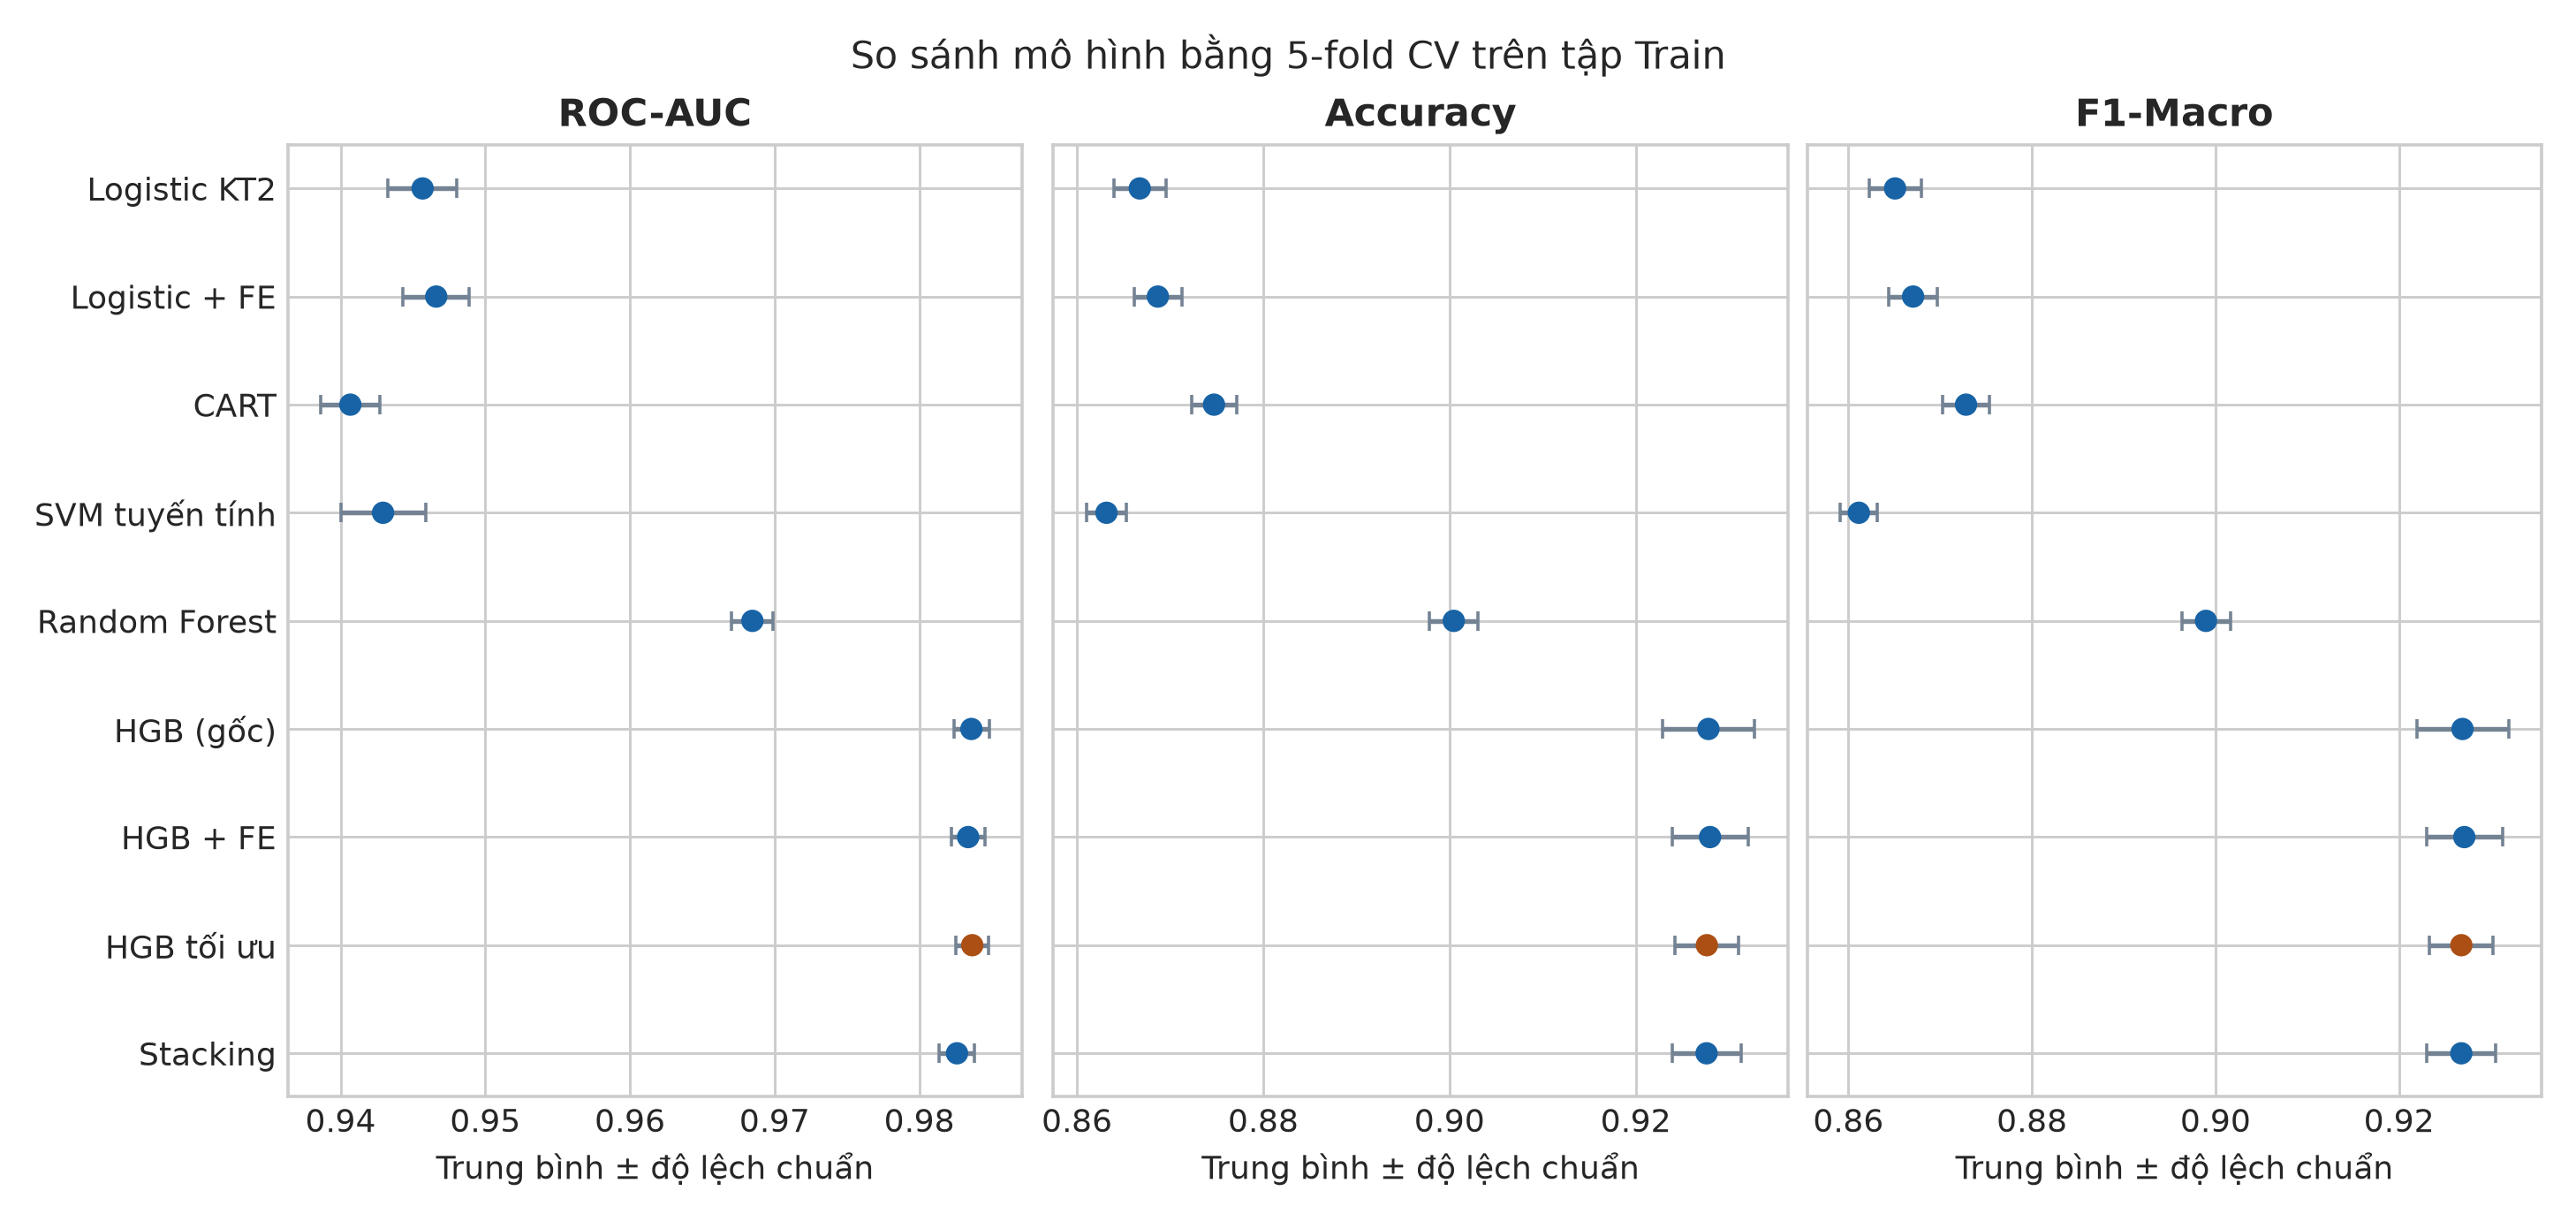
\includegraphics[width=\linewidth]{so_sanh_mo_hinh_kt2_vs_kt3.png}
  \caption{So sánh các mô hình theo ba chỉ số trên 5-fold CV}
  \label{fig:cv}
\end{figure}

Hình~\ref{fig:cv} cho thấy CART có Accuracy cao hơn Logistic KT2 trong khi ROC-AUC thấp hơn. Accuracy đánh giá nhãn dự đoán ở ngưỡng hiện hành, còn ROC-AUC đánh giá thứ hạng của điểm dự đoán. Random Forest và các cấu hình HGB vượt đối chứng trên cả ba chỉ số. Theo tiêu chí ROC-AUC đã chọn, \KTFinalModel\ đứng đầu bảng.

\section{Kết quả tìm kiếm siêu tham số}

GridSearchCV xét 24 tổ hợp từ tốc độ học $\{0{,}05;0{,}08;0{,}12\}$, độ sâu tối đa $\{6;8\}$, số vòng lặp $\{150;200\}$ và hệ số L2 $\{0;0{,}5\}$. Tất cả ứng viên dùng cùng fold và cùng hàm chấm ROC-AUC. Quy tắc chọn mô hình cuối là ROC-AUC trung bình cao nhất từ CV. Sau khi cố định lựa chọn, script fit các pipeline trên 35.000 mẫu Train và mới đánh giá mô hình đã chọn cùng đối chứng trên Test.

GridSearchCV chọn tốc độ học \KTBestRate, độ sâu tối đa \KTBestDepth, số vòng lặp \KTBestIter\ và hệ số L2 \KTBestLTwo. Bảng~\ref{tab:grid} ghi năm cấu hình đầu trong \KTGridSize\ tổ hợp. Toàn bộ cấu hình, thứ hạng và độ lệch chuẩn được lưu trong tệp JSON.

\begin{table}[H]
  \caption{Năm cấu hình đầu của GridSearchCV trên tập Train}
  \label{tab:grid}
  \begin{tabularx}{\textwidth}{|X|r|r|r|r|r|}
    \hline
    \textbf{Hạng} & \textbf{Tốc độ học} & \textbf{Độ sâu} & \textbf{Số vòng} & \textbf{L2} & \textbf{ROC-AUC CV} \\
    \hline
    \KTGridRows
  \end{tabularx}
\end{table}

Điểm CV của cấu hình tối ưu sử dụng cùng các fold đã dùng để chọn phương án. Vì vậy, điểm này được đọc cùng kết quả trên Validation và Test. Lưới tìm kiếm giới hạn phạm vi kết luận về cấu hình phù hợp trong thực nghiệm này.

\section{Nghiên cứu bóc tách trên tập Train}

Bảng~\ref{tab:ablation} lấy kết quả cấu hình sau trừ cấu hình trước trên cùng các fold. Khi khảo sát đặc trưng, mô hình và siêu tham số được giữ cố định. Các hàng thay thuật toán hoặc tinh chỉnh siêu tham số giữ nguyên tập đặc trưng. So sánh Stacking với HGB đo ảnh hưởng của việc thay bằng thiết kế tổ hợp đã xây dựng.

\begin{table}[H]
  \caption{Ablation theo từng cặp trên cùng 5-fold CV}
  \label{tab:ablation}
  \begin{tabularx}{\textwidth}{|>{\raggedright\arraybackslash}X|r|r|r|r|r|}
    \hline
    \textbf{Thay đổi} & \textbf{AUC trước} & \textbf{AUC sau} & \textbf{$\Delta$ AUC} & \textbf{$\Delta$ Acc.} & \textbf{$\Delta$ F1} \\
    \hline
    \KTAblationRows
  \end{tabularx}
  \par\smallskip\footnotesize $\Delta$ Acc. tính bằng điểm phần trăm. AUC là ROC-AUC. F1 là F1-Macro.
\end{table}

\begin{figure}[H]
  \centering
  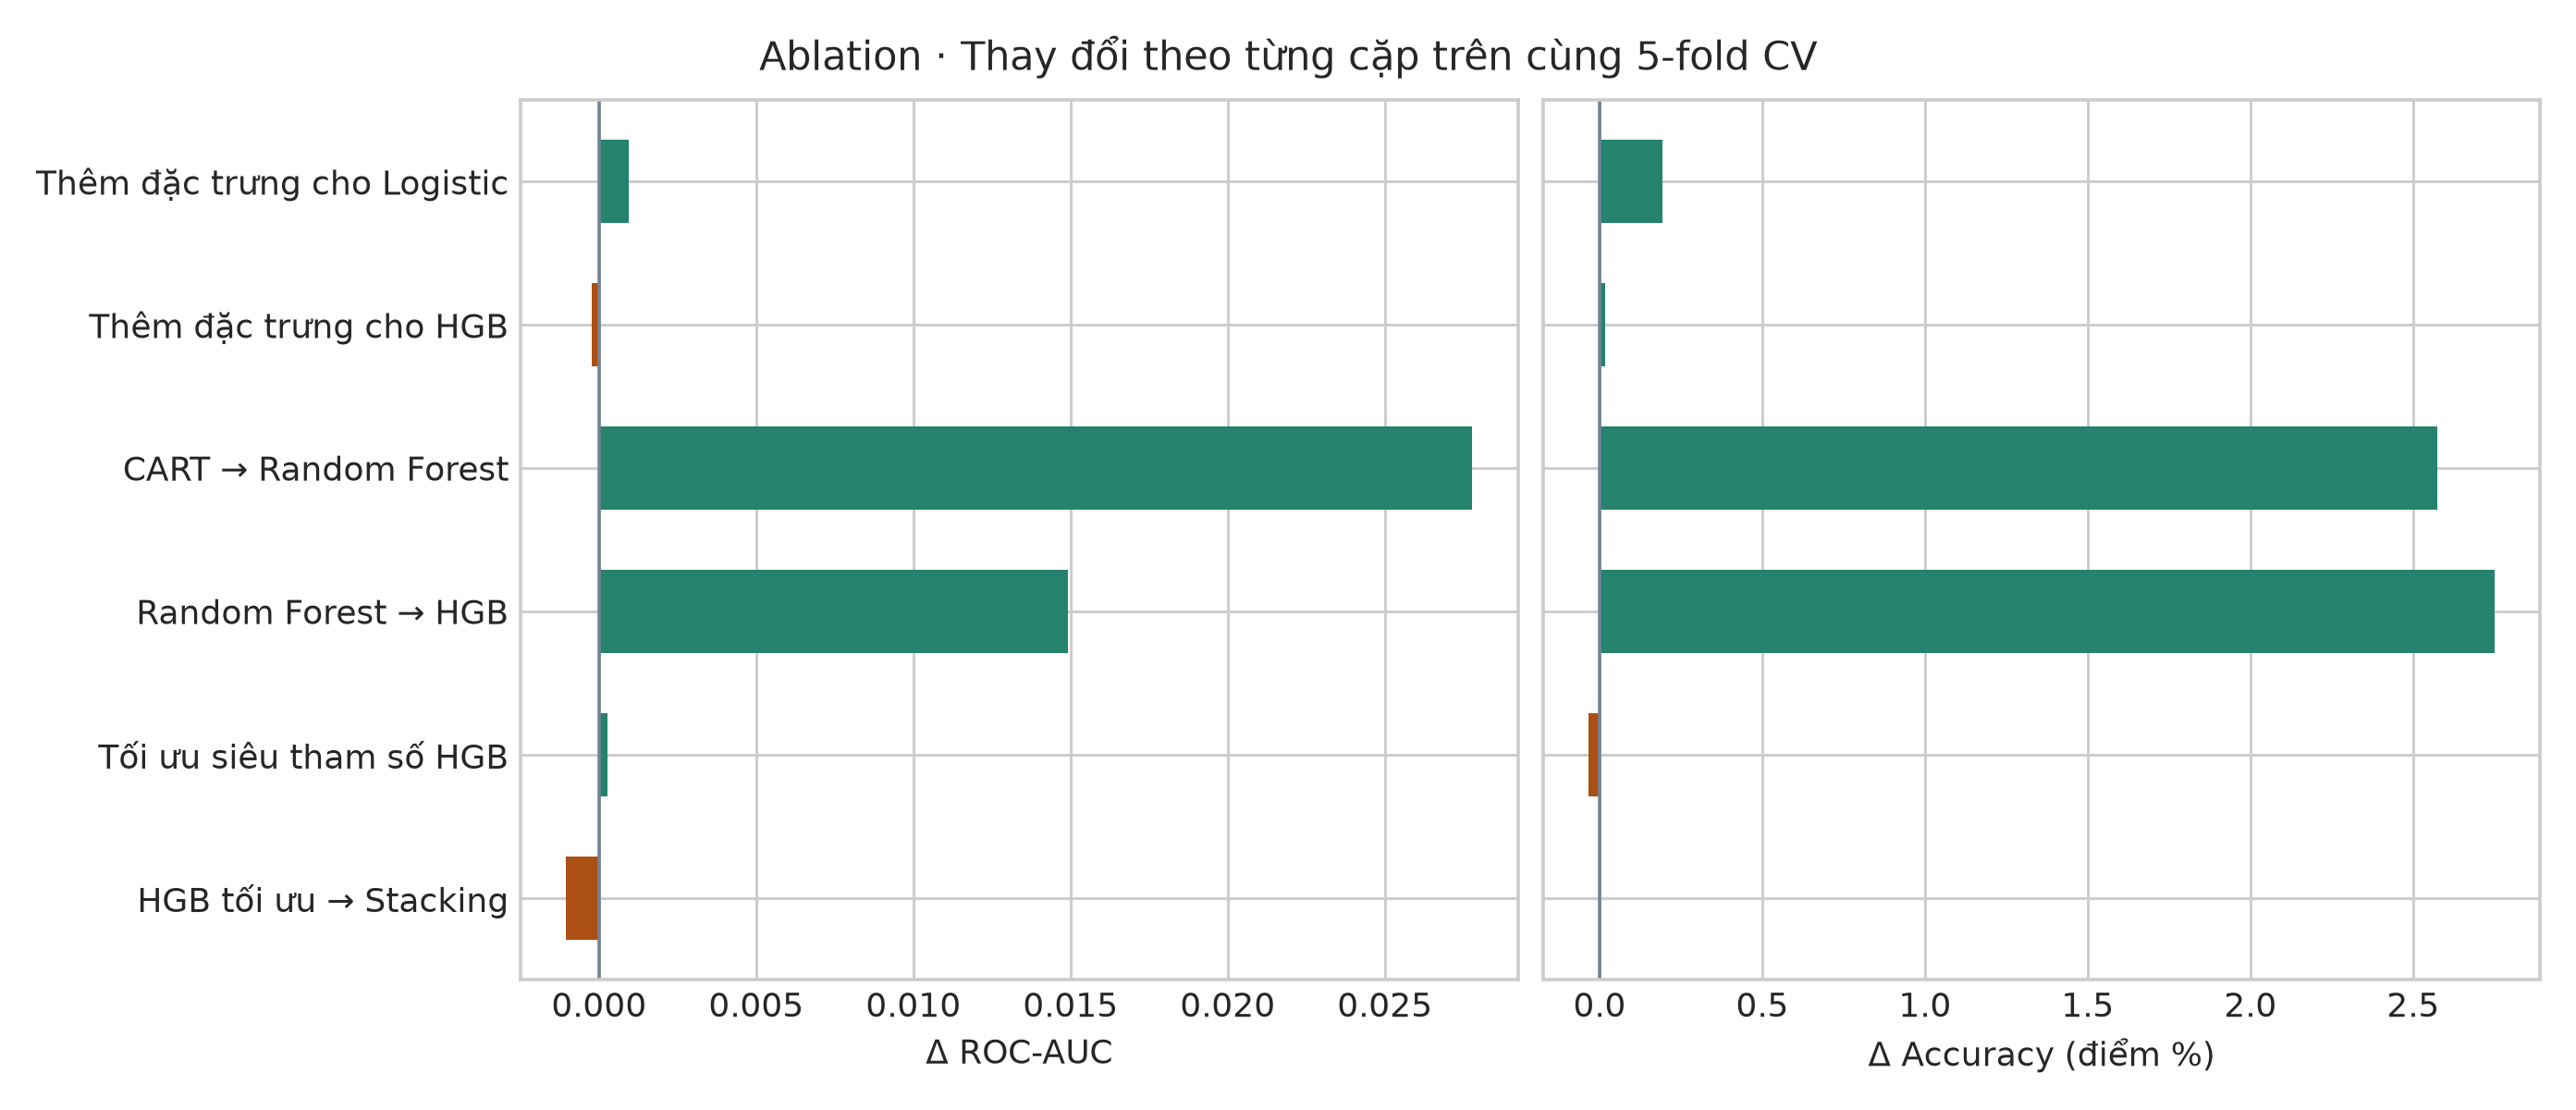
\includegraphics[width=\linewidth]{ablation_study_kt3.png}
  \caption{Chênh lệch ROC-AUC và Accuracy ở từng cặp đối chứng}
  \label{fig:ablation}
\end{figure}

Bổ sung đặc trưng làm ROC-AUC của Logistic thay đổi \KTLogisticFEDelta, và của HGB cấu hình gốc thay đổi \KTHGBFEDelta. Tìm siêu tham số trên HGB có đặc trưng mới làm ROC-AUC thay đổi \KTHGBTuningDelta. Mức chênh này nhỏ so với chênh lệch giữa các họ mô hình trên Hình~\ref{fig:ablation}. Stacking tăng độ phức tạp và có ROC-AUC thấp hơn HGB tối ưu. Kết quả cho thấy lợi ích đo được của các đặc trưng phụ thuộc cấu hình và chỉ số đánh giá.

\section{Khả năng tổng quát hóa của mô hình đã chốt}

\begin{table}[H]
  \caption{Đối chiếu kiểm định chéo, Validation và Test}
  \label{tab:generalization}
  \begin{tabularx}{\textwidth}{|X|r|r|r|r|r|r|}
    \hline
    \textbf{Mô hình} & \textbf{AUC CV} & \textbf{Std CV} & \textbf{AUC Val} & \textbf{AUC Test} & \textbf{Acc. Test} & \textbf{F1 Test} \\
    \hline
    \KTGeneralizationRows
  \end{tabularx}
\end{table}

\begin{table}[H]
  \caption{Chỉ số bổ sung trên 7.500 hồ sơ Test}
  \label{tab:extra-test}
  \begin{tabularx}{\textwidth}{|X|r|r|r|r|r|r|}
    \hline
    \textbf{Mô hình} & \textbf{AP} & \textbf{Precision} & \textbf{Recall} & \textbf{Specificity} & \textbf{FP} & \textbf{FN} \\
    \hline
    \KTExtraTestRows
  \end{tabularx}
\end{table}

\KTFinalModel\ đạt ROC-AUC \KTFinalCV\ trên CV, \KTFinalVal\ trên Validation và \KTFinalTest\ trên Test. Chênh lệch tuyệt đối CV--Test là \KTCVTestGap. Độ lệch chuẩn ROC-AUC qua 5 fold là \KTFinalCVStd. Điểm ROC-AUC trung bình trên phần huấn luyện của các fold là \KTFinalTrainAUC, cách Test \KTTrainTestGap. Các kết quả mô tả độ ổn định trong phân hoạch dữ liệu này và vùng dữ liệu mô phỏng đang xét.

Accuracy trên Test tăng từ \KTBaseAcc\ lên \KTFinalAcc, với F1-Macro \KTFinalFscore. Tổng số dự đoán sai giảm từ \KTBaseErrors\ xuống \KTFinalErrors, giảm \KTErrorsReduced\ hồ sơ (\KTErrorsReducedPct). Hai loại lỗi được trình bày riêng trong Bảng~\ref{tab:extra-test} và Hình~\ref{fig:confusion}.

\section{Trực quan hóa và giải thích}

\subsection{Đường ROC, Precision--Recall và ma trận nhầm lẫn}

\begin{figure}[H]
  \centering
  \begin{minipage}[t]{0.485\linewidth}
    \centering
    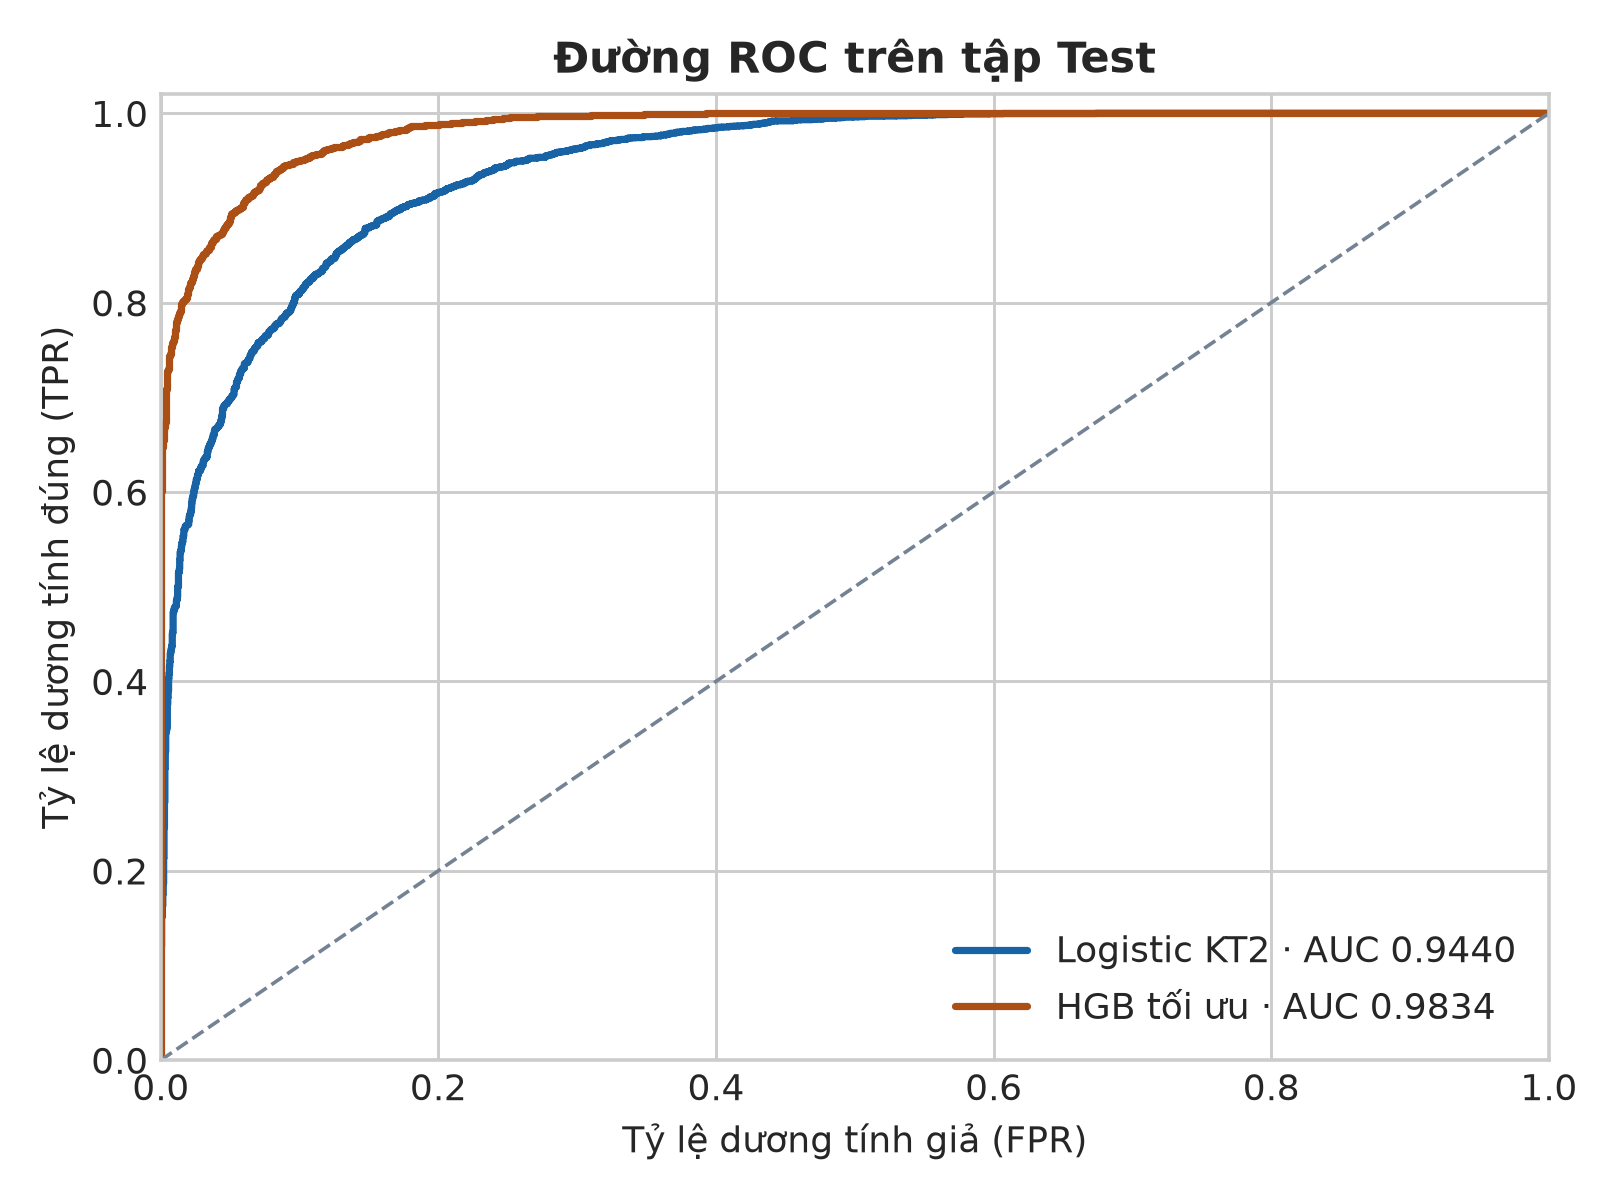
\includegraphics[width=\linewidth]{duong_cong_roc_so_sanh_kt3.png}
    \caption{Đường ROC trên tập Test}
    \label{fig:roc}
  \end{minipage}\hfill
  \begin{minipage}[t]{0.485\linewidth}
    \centering
    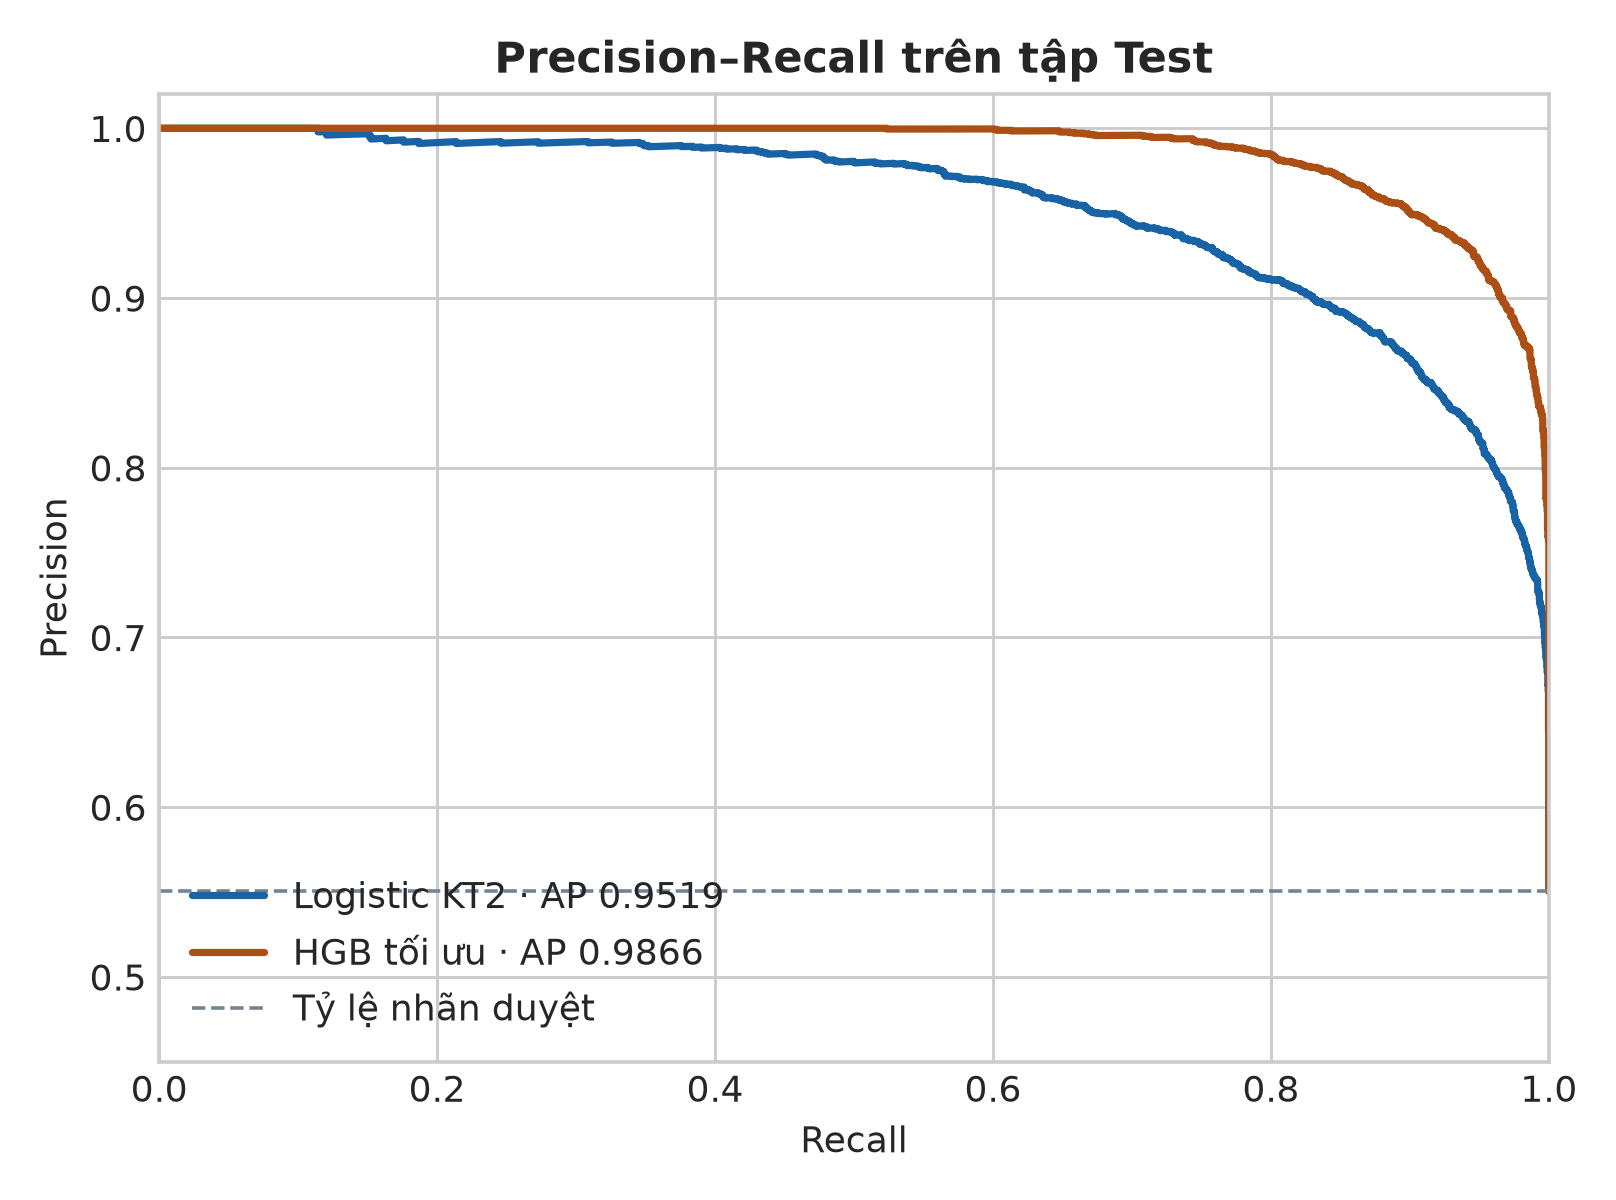
\includegraphics[width=\linewidth]{duong_cong_pr_so_sanh_kt3.png}
    \caption{Đường Precision--Recall trên tập Test}
    \label{fig:pr}
  \end{minipage}
\end{figure}

Trên Hình~\ref{fig:roc}, đường của HGB nằm cao hơn rõ rệt so với Logistic KT2 ở vùng FPR thấp. Hình~\ref{fig:pr} cho thấy HGB duy trì Precision cao hơn khi tăng Recall trong phần lớn khoảng khảo sát, với AP \KTFinalPR. Hai đường sử dụng điểm liên tục và thể hiện đánh đổi khi thay ngưỡng.

\begin{figure}[H]
  \centering
  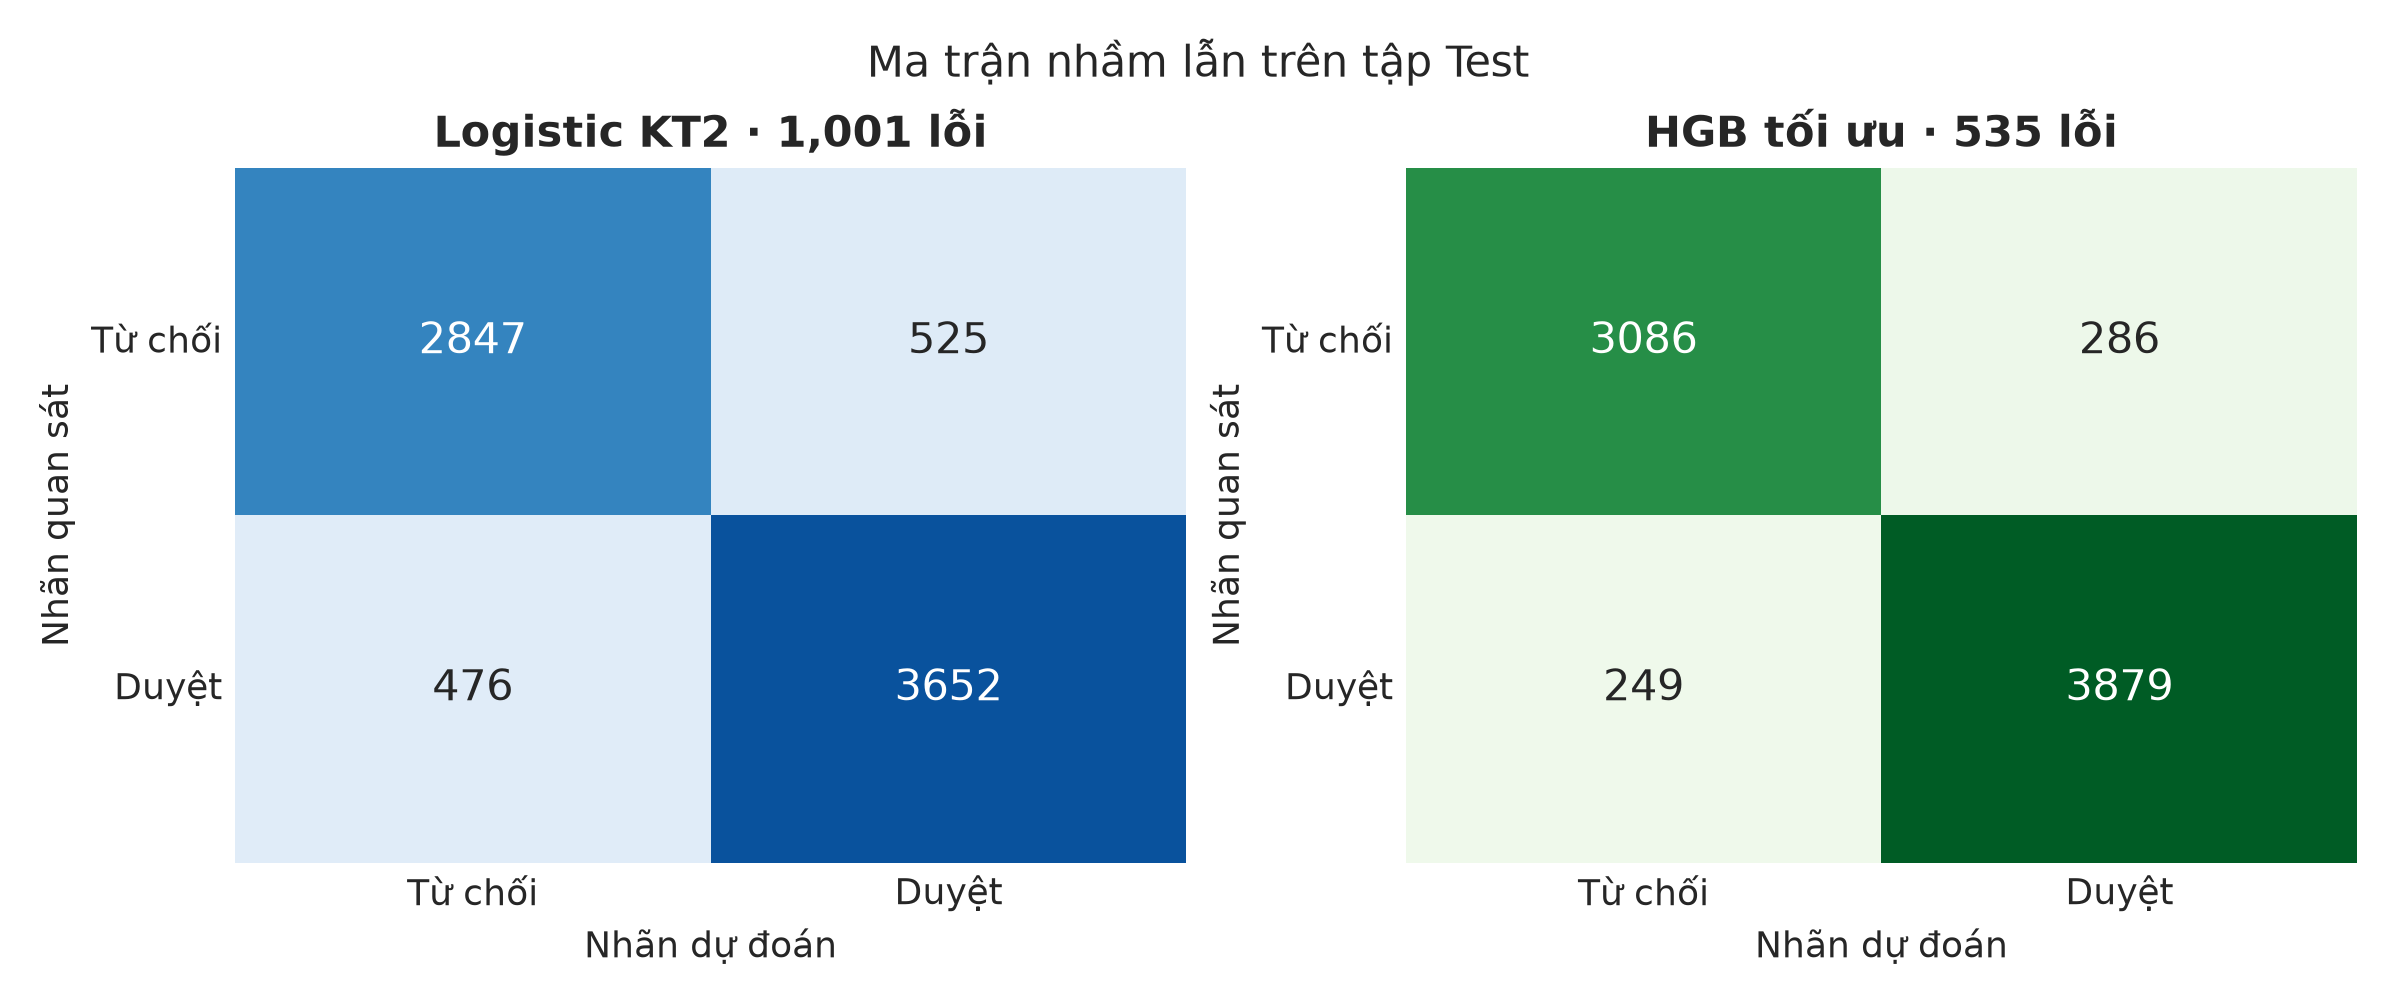
\includegraphics[width=\linewidth]{ma_tran_nham_lan_kt2_vs_kt3.png}
  \caption{Ma trận nhầm lẫn của đối chứng và mô hình đã chọn trên Test}
  \label{fig:confusion}
\end{figure}

Ma trận tại ngưỡng mặc định cho thấy FP giảm từ \KTBaseFP\ xuống \KTFinalFP, còn FN giảm từ \KTBaseFN\ xuống \KTFinalFN. Với bài toán này, FP và FN được xác định theo nhãn duyệt hoặc từ chối của bộ dữ liệu.

\subsection{Độ quan trọng đặc trưng}

\begin{figure}[H]
  \centering
  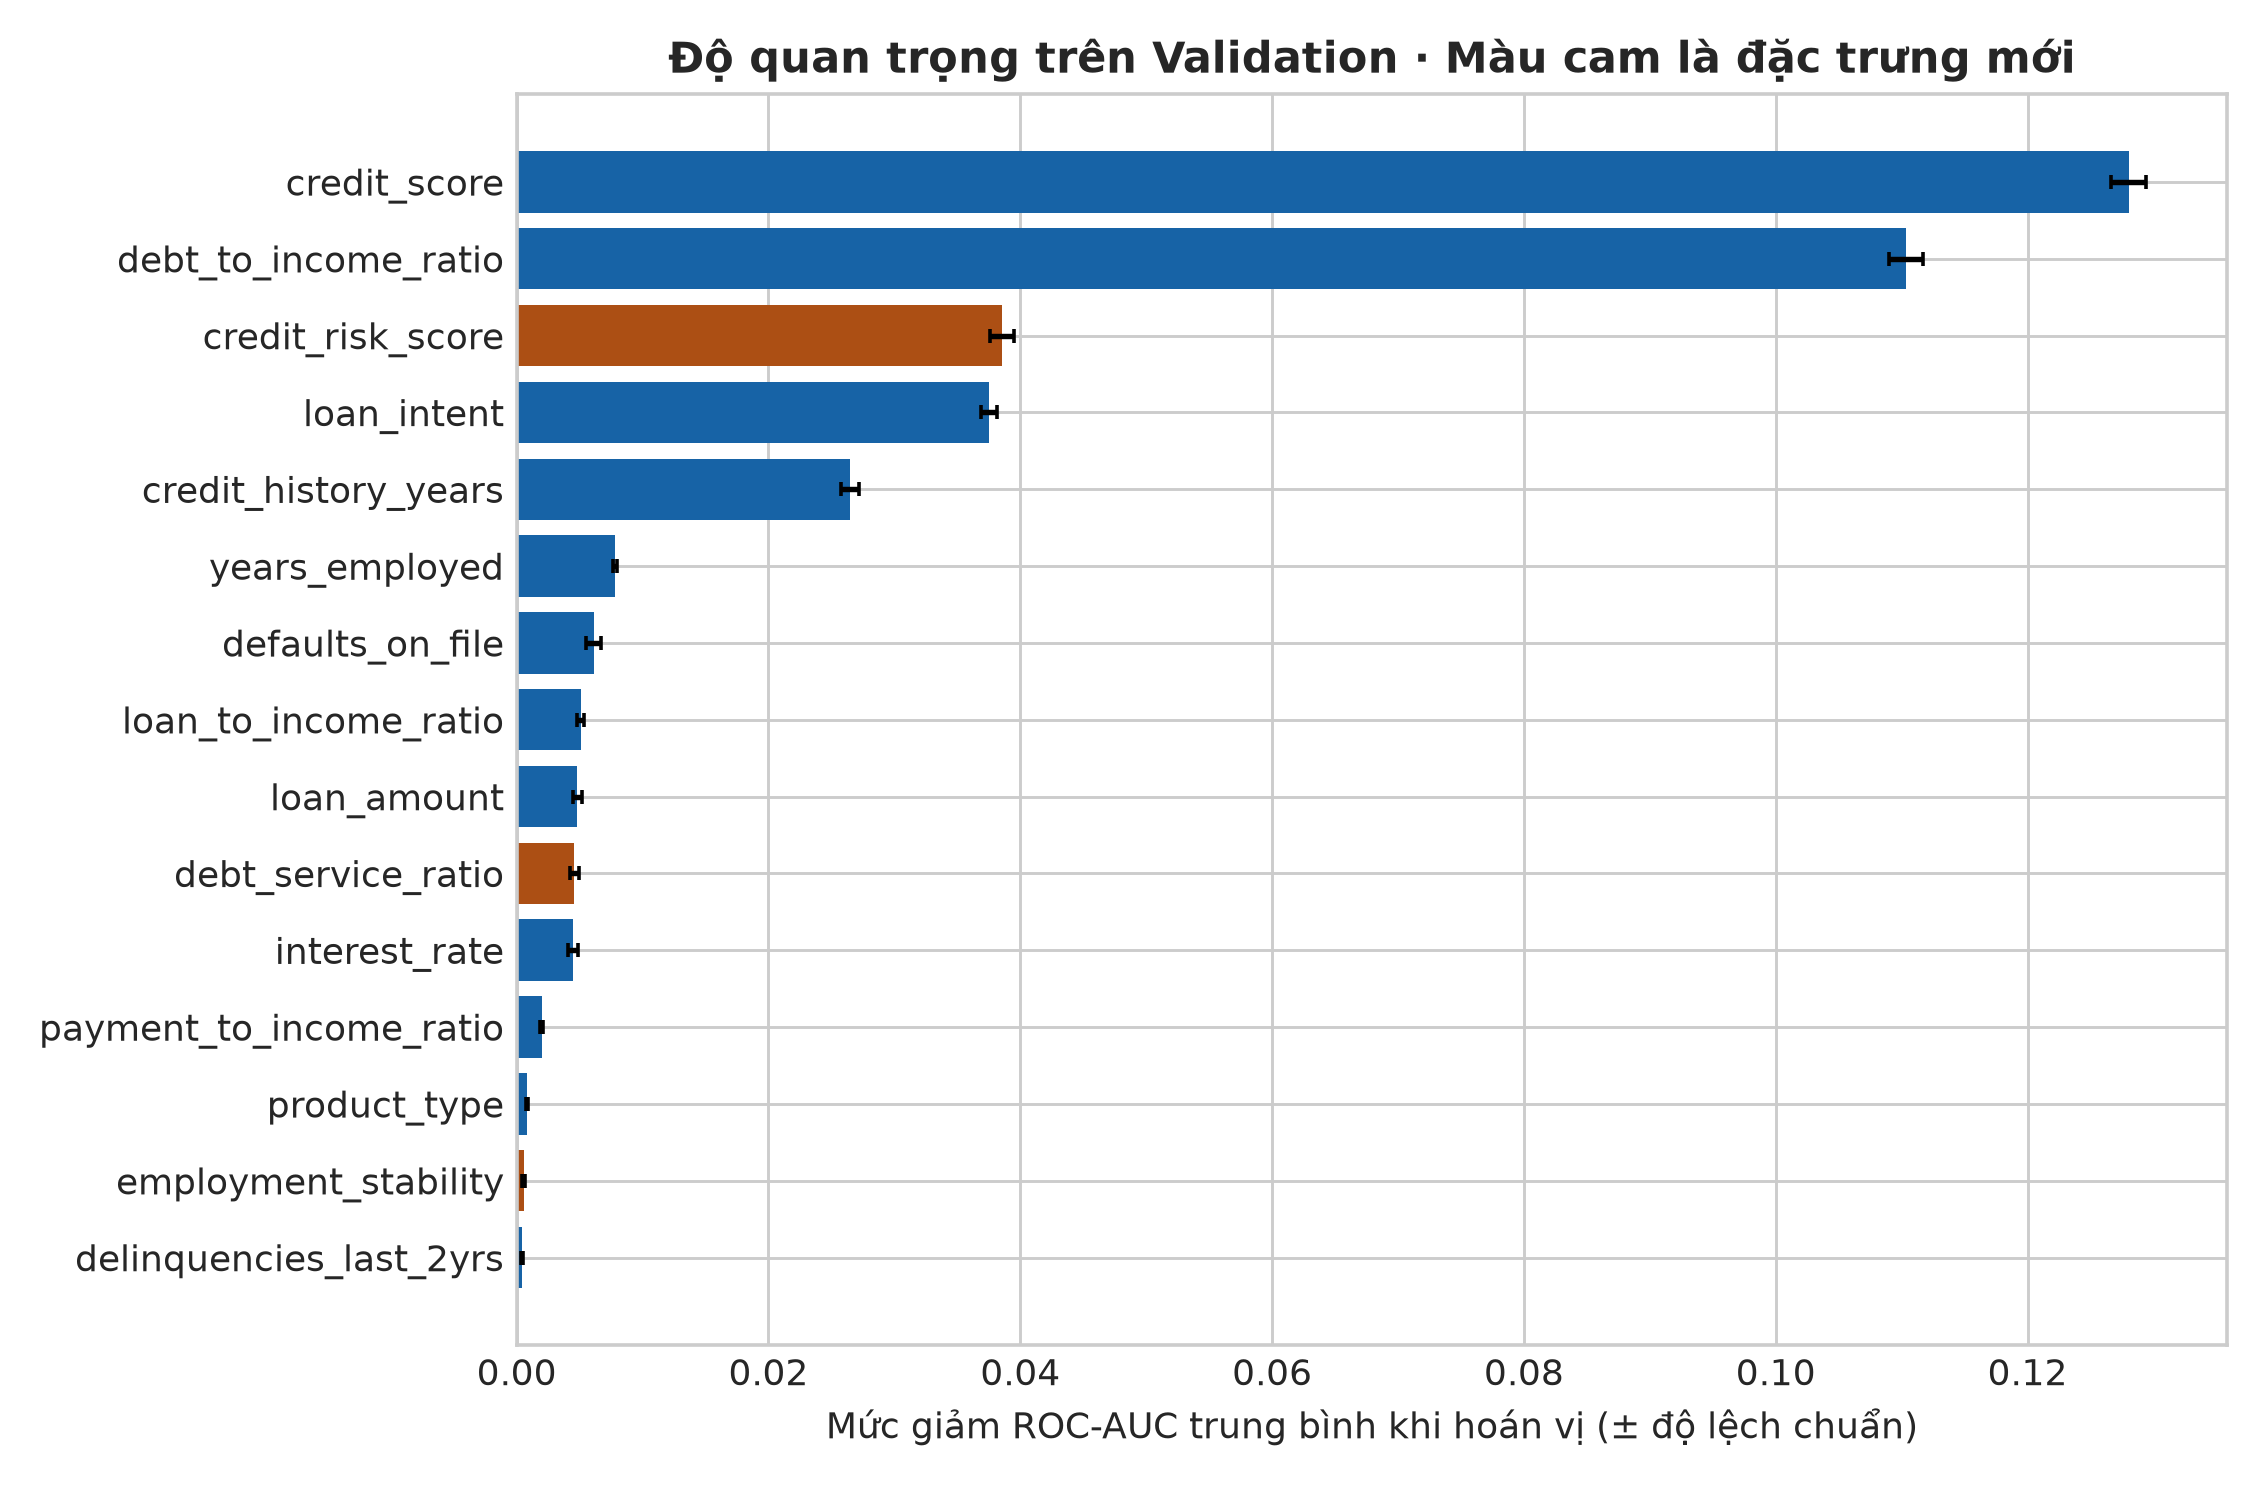
\includegraphics[width=0.93\linewidth]{do_quan_trong_dac_trung_kt3.png}
  \caption{Độ quan trọng theo hoán vị trên Validation}
  \label{fig:importance}
\end{figure}

Mỗi đặc trưng được hoán vị 5 lần độc lập trên Validation. Hình~\ref{fig:importance} hiển thị mức giảm ROC-AUC trung bình và độ lệch chuẩn của 15 đặc trưng có ảnh hưởng lớn nhất. \KTLeadingFeature\ đứng đầu với mức giảm trung bình \KTLeadingFeatureImpact. Hoán vị phản ánh mức phụ thuộc của mô hình trong tập này. Các biến tương quan có thể san sẻ thông tin và làm thay đổi thứ hạng khi hoán vị từng cột.

\subsection{Đường cong kiểm định và đường cong học tập}

\begin{figure}[H]
  \centering
  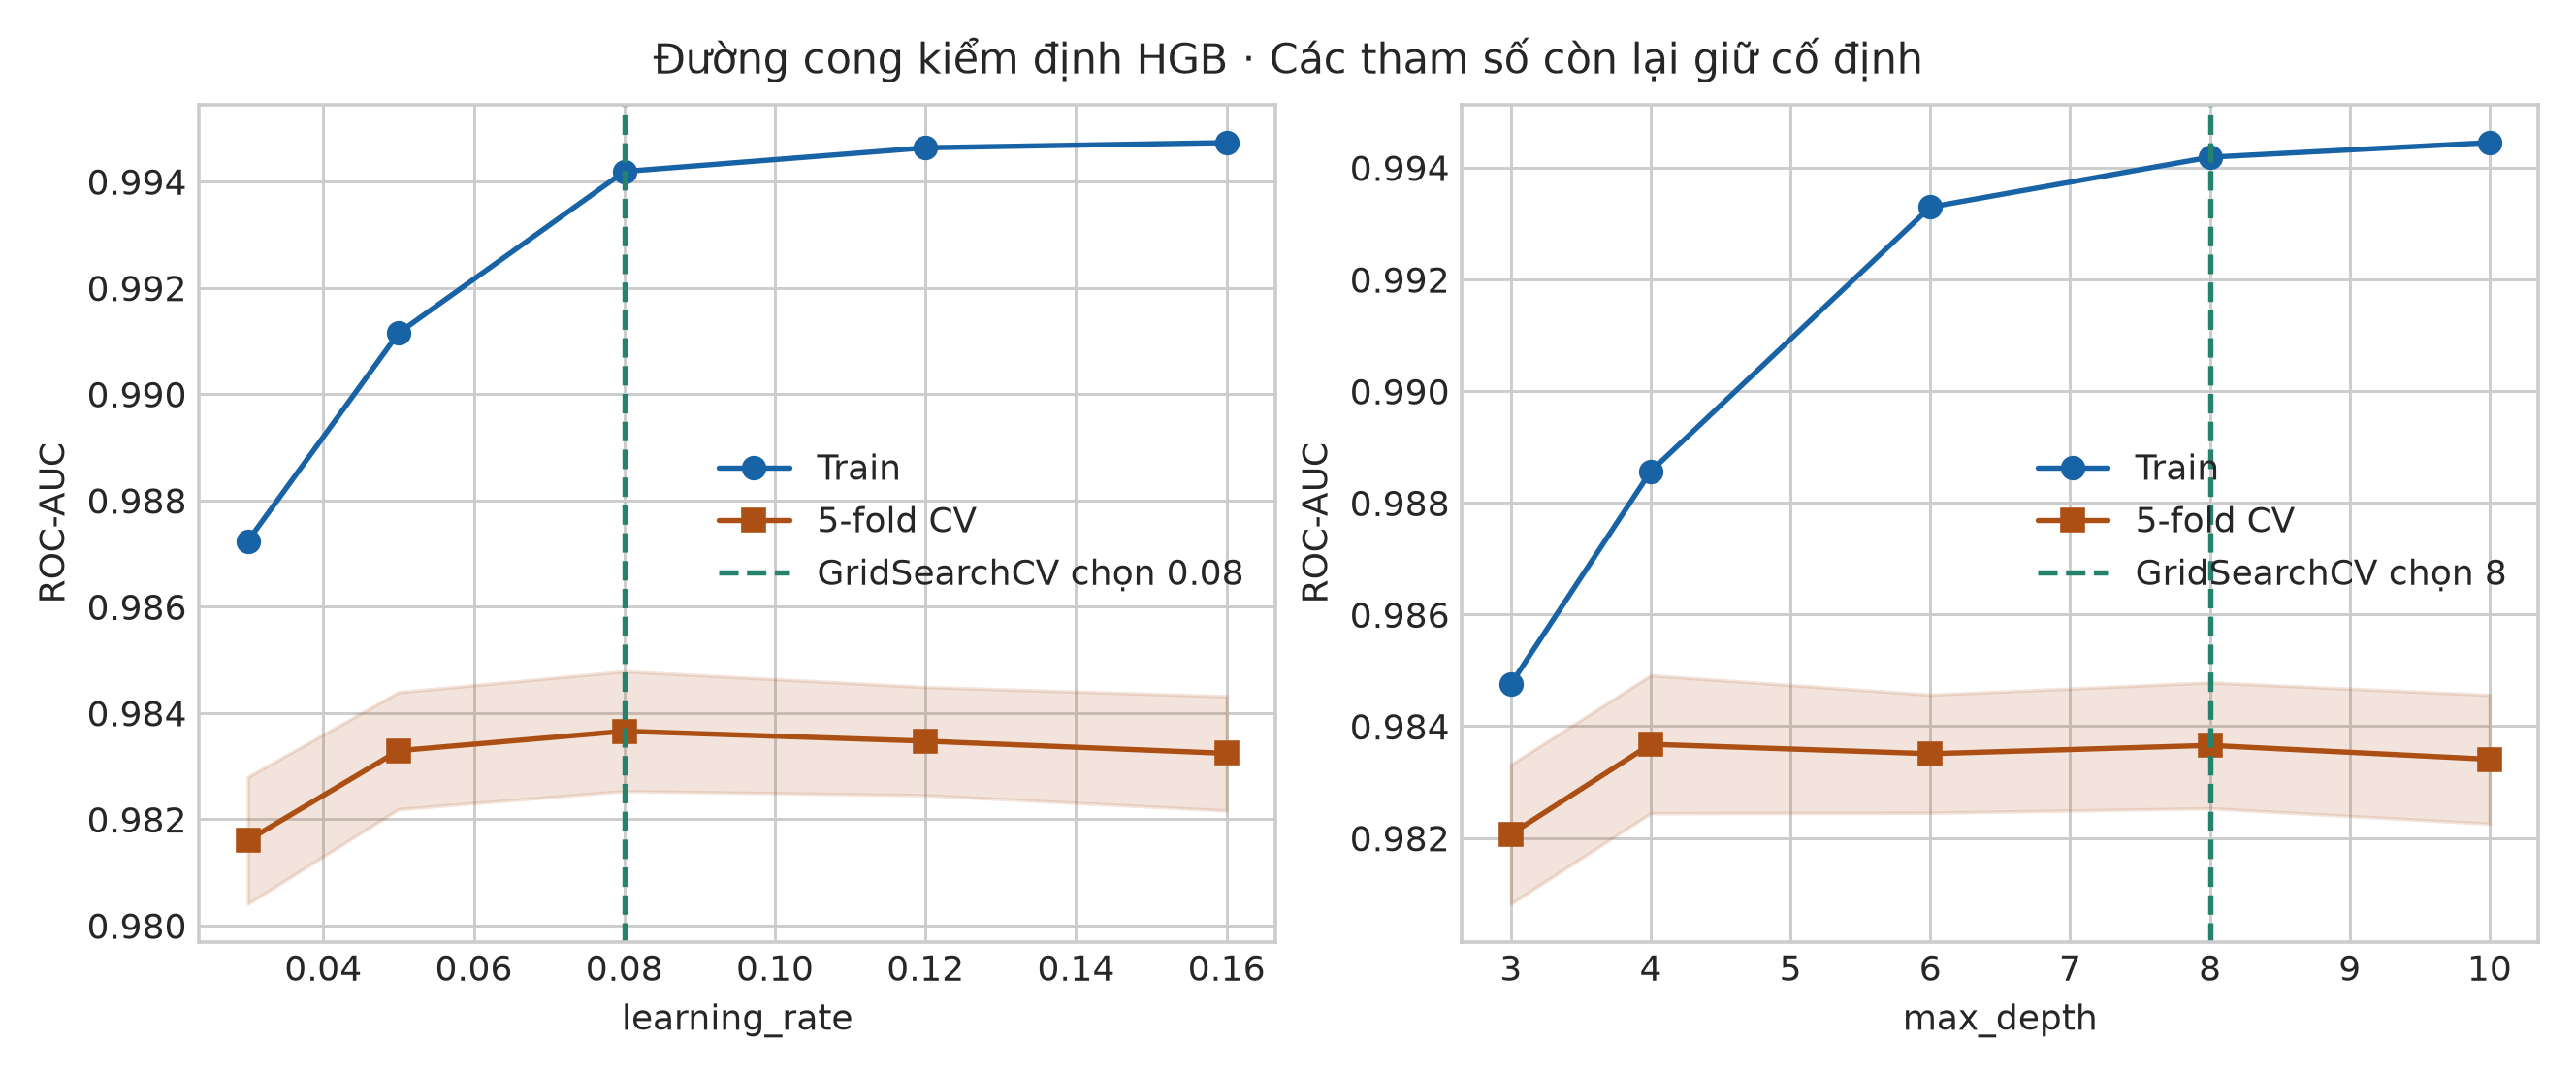
\includegraphics[width=\linewidth]{duong_cong_kiem_dinh_hyperparameter.png}
  \caption{Độ nhạy của HGB theo tốc độ học và độ sâu tối đa}
  \label{fig:validation-curves}
\end{figure}

Hình~\ref{fig:validation-curves} thay đổi lần lượt tốc độ học và độ sâu. Các tham số còn lại giữ ở cấu hình GridSearchCV đã chọn. Pipeline là đối tượng được kiểm định nên mỗi fold fit tiền xử lý riêng. Ở lát cắt độ sâu, cấu hình 4 và 8 có ROC-AUC kiểm định gần bằng nhau, trong khi ROC-AUC trên Train tiếp tục tăng. Độ sâu 4 là điểm khảo sát bổ sung ngoài lưới chính thức. Kết quả được dùng để giải thích độ nhạy của mô hình.

\begin{figure}[H]
  \centering
  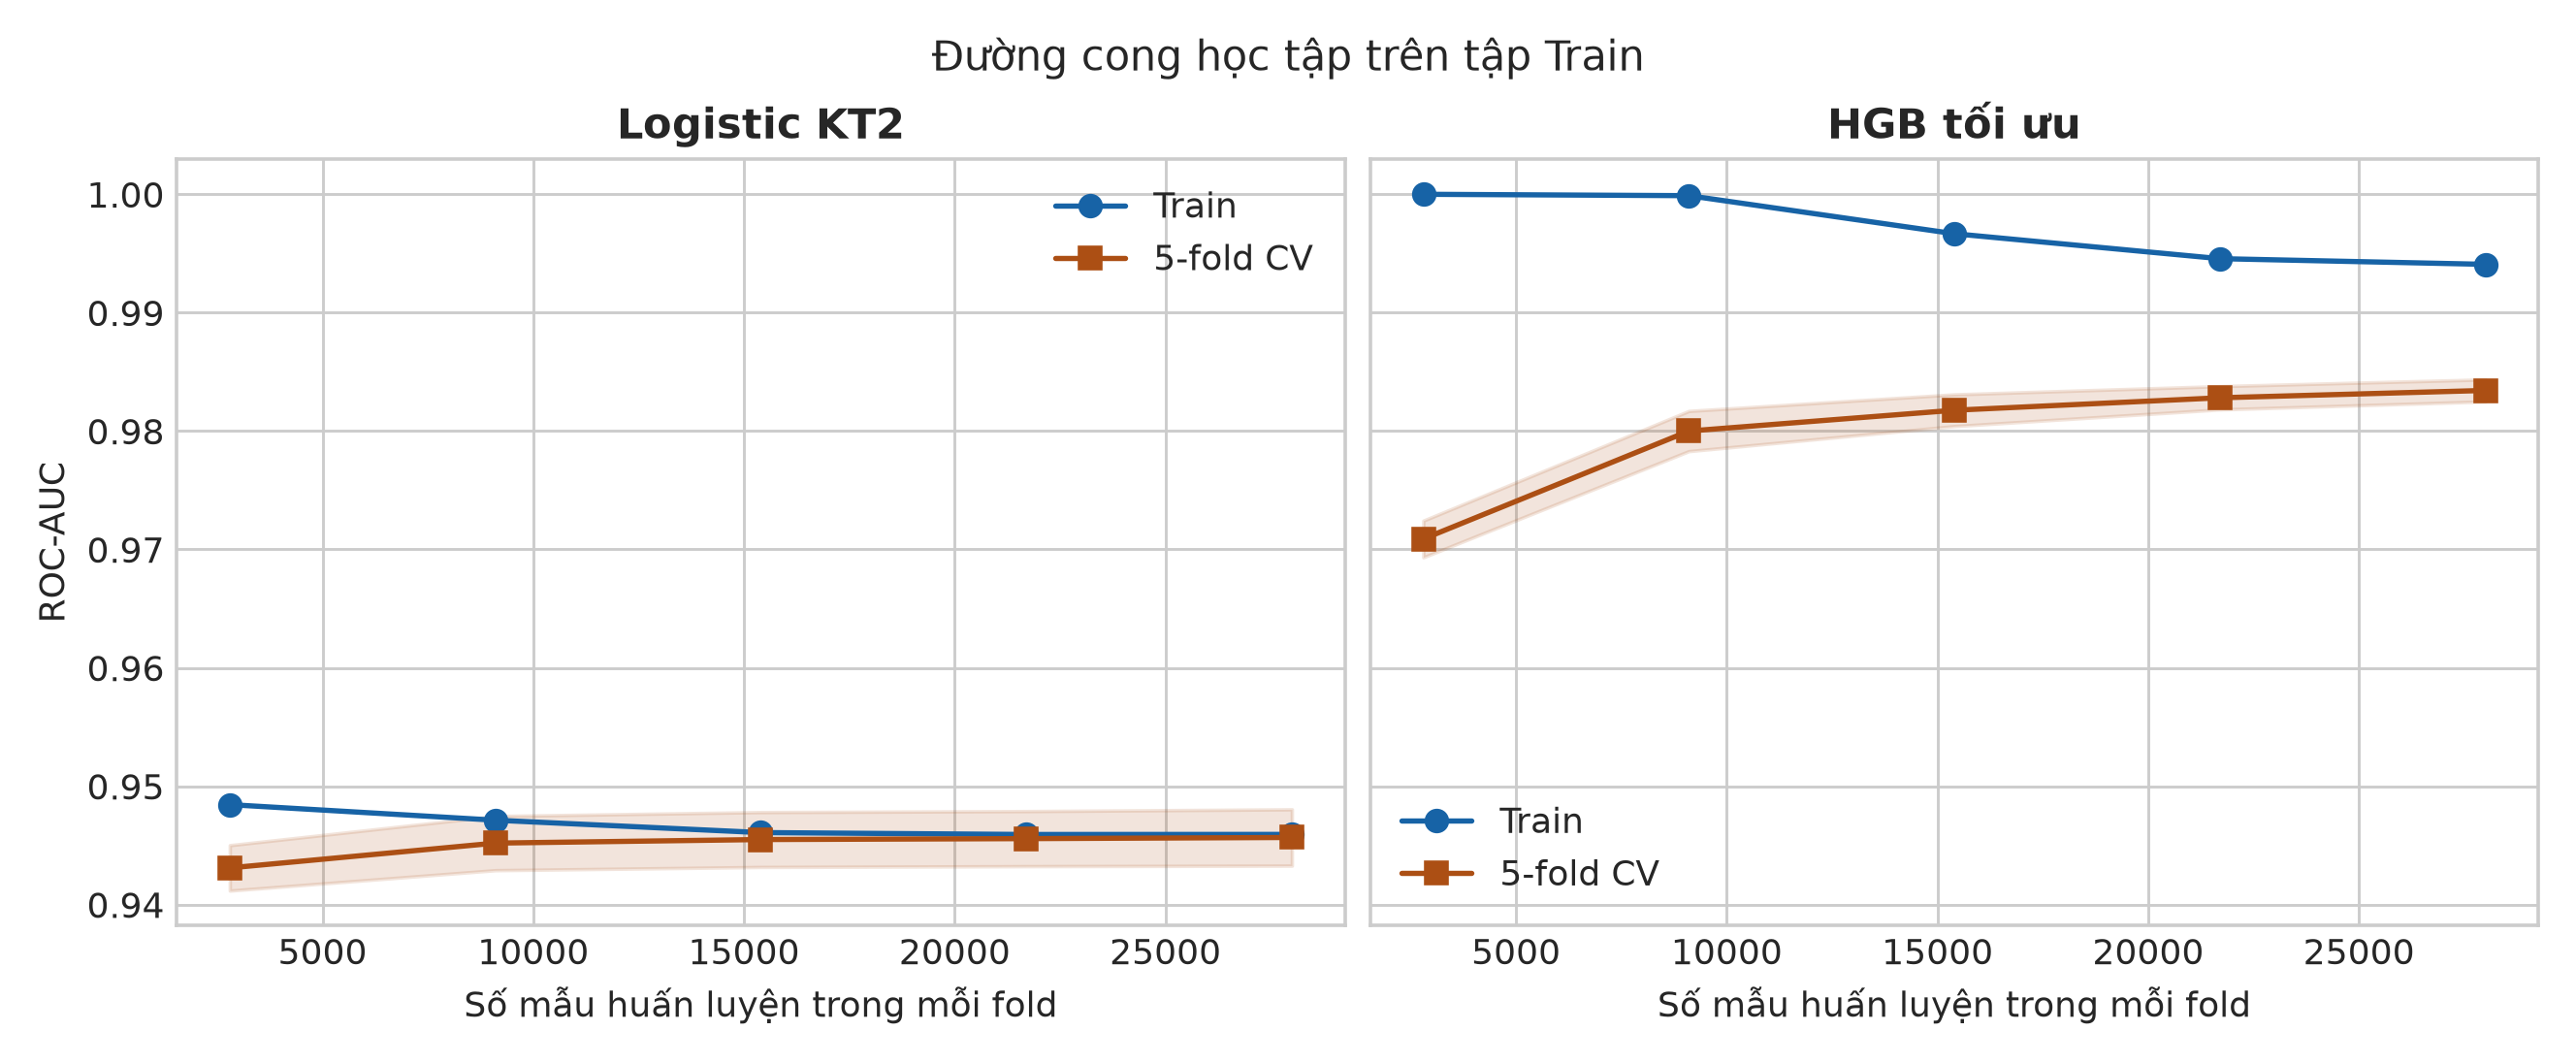
\includegraphics[width=\linewidth]{duong_cong_hoc_tap_kt3.png}
  \caption{Đường cong học tập của Logistic Regression và mô hình đã chọn}
  \label{fig:learning}
\end{figure}

Trong Hình~\ref{fig:learning}, đường kiểm định của Logistic thay đổi ít khi tăng kích thước mẫu. HGB đạt ROC-AUC kiểm định cao hơn, đồng thời thể hiện khoảng cách Train--CV rõ hơn so với Logistic. Kết quả gợi ý rằng thay đổi họ mô hình giải quyết được một phần giới hạn của biên tuyến tính.

\section{Đánh đổi và lựa chọn mô hình}

\begin{table}[H]
  \caption{So sánh ứng viên theo hiệu năng, độ ổn định, độ trễ và diễn giải}
  \label{tab:tradeoff}
  \begin{tabularx}{\textwidth}{|l|r|r|r|r|>{\raggedright\arraybackslash}X|}
    \hline
    \textbf{Mô hình} & \textbf{AUC CV} & \textbf{Std CV} & \textbf{AUC Val} & \textbf{ms/1.000 mẫu} & \textbf{Diễn giải} \\
    \hline
    \KTTradeoffRows
  \end{tabularx}
\end{table}

\KTFinalModel\ đứng đầu theo ROC-AUC trung bình trên CV. Mô hình HGB dùng đặc trưng gốc có điểm gần với cấu hình được chọn. Điều này cho thấy có thể cân nhắc phương án ít đặc trưng hơn nếu ưu tiên vận hành gọn. Logistic thuận tiện khi cần đọc trực tiếp hướng tác động của hệ số. Stacking tốn thêm các mô hình tầng một và tầng hai, trong khi kết quả CV chưa cải thiện so với HGB tối ưu.

\unnumberedchapter{KẾT LUẬN VÀ HƯỚNG PHÁT TRIỂN}

Trên bộ dữ liệu 50.000 hồ sơ, \KTFinalModel\ được chọn bằng 5-fold CV trên Train. Trên 7.500 mẫu Test, mô hình đạt ROC-AUC \KTFinalTest, Accuracy \KTFinalAcc\ và F1-Macro \KTFinalFscore. So với Logistic KT2, số lỗi giảm \KTErrorsReduced\ hồ sơ. Các cặp ablation cho thấy thay đổi họ mô hình tạo chênh lệch lớn hơn thiết kế đặc trưng và tinh chỉnh HGB trong phạm vi đã khảo sát.

Kết quả phản ánh hiệu năng trên dữ liệu mô phỏng. Ở giai đoạn tiếp theo, nhóm có thể đánh giá trên một nguồn dữ liệu độc lập, kiểm tra khả năng sử dụng các biến tại đúng thời điểm ra quyết định, và bổ sung giải thích theo từng hồ sơ. Định mức chi phí FP và FN cũng giúp chọn ngưỡng vận hành có căn cứ.

\begin{thebibliography}{9}

\bibitem{kaggle}
Parth Patel2130, \textit{Realistic Loan Approval Dataset | US \& Canada}, Kaggle, 2025.
Tệp \texttt{Loan\_approval\_data\_2025.csv}, giấy phép \href{https://creativecommons.org/licenses/by-nc/4.0/}{CC BY-NC 4.0}.
\href{https://www.kaggle.com/datasets/parthpatel2130/realistic-loan-approval-dataset-us-and-canada}{Trang dữ liệu trên Kaggle}.

\bibitem{cart}
L. Breiman, J. H. Friedman, R. A. Olshen và C. J. Stone,
\textit{Classification and Regression Trees}, Wadsworth, 1984.

\bibitem{breiman}
L. Breiman, \textit{Random Forests}, Machine Learning, tập 45, tr. 5--32, 2001.

\bibitem{friedman}
J. H. Friedman, \textit{Greedy Function Approximation: A Gradient Boosting Machine},
The Annals of Statistics, tập 29, số 5, tr. 1189--1232, 2001.

\bibitem{wolpert}
D. H. Wolpert, \textit{Stacked Generalization}, Neural Networks, tập 5, số 2,
tr. 241--259, 1992.

\bibitem{sklearn}
F. Pedregosa và cộng sự, \textit{Scikit-learn: Machine Learning in Python},
Journal of Machine Learning Research, tập 12, tr. 2825--2830, 2011.

\bibitem{course}
Bộ môn Học máy, Khoa Công nghệ Thông tin, ICTU.
Bài giảng Học máy, Bài 2, Bài 4, Bài 6, Bài 7 và Bài 9.

\bibitem{kt2}
\nhom, \textit{Mã nguồn mô hình đối chứng và phân hoạch dữ liệu Bài kiểm tra 2 (KT2)}, GitHub, 2026.
\url{https://github.com/luongchiconghash/Nhom_13/tree/main/Kiemtra2/code}.

\end{thebibliography}

\end{document}
